\chapter{设计模式}

\section{设计模式}

\subsection{设计模式(Design Pattern)}

设计模式代表了最佳的实践,通常被有经验的面向对象软件开发人员所采用。设计模式是开发人员在开发过程中面临的一般问题的解决方案,这些解决方案是众多开发人员经过相当长一段时间的试验和错误总结出来的。\\

设计模式是一套被反复使用的、多数人知晓的、经过分类编目的、代码设计经验的总结。使用设计模式是为了重用代码、让代码更容易被他人理解、保证代码可靠性。设计模式使代码编制真正工程化,是软件工程的基石。项目中合理地运用设计模式可以完美地解决很多问题,每种模式在现实中都有相应的原理来与之对应,每种模式都描述了周围不断重复发生的问题,以及该问题的核心解决方案,这也是设计模式能被广泛应用的原因。\\

\subsection{GOF(Gang of Four)}

1994年,由Erich Gamma、Richard Helm、Ralph Johnson和John Vlissides四人合著出版了一本名为Design Patterns - Elements of Reusable Object-Oriented Software的书,该书首次提到了软件开发中设计模式的概念。\\

四位作者合称GOF,他们所提出的设计模式主要基于两个面向对象设计原则:

\begin{enumerate}
    \item 对接口编程而不是对实现编程。
    \item 优先使用对象组合而不是继承。
\end{enumerate}

\vspace{0.5cm}

\subsection{设计模式分类}

Design Patterns - Elements of Reusable Object-Oriented Software中提到的设计模式可以分为三大类:

\begin{enumerate}
    \item 创建型模式(creational patterns):提供了一种在创建对象的同时隐藏创建逻辑的方式,主要特点是将对象的创建与使用分离。
          \begin{itemize}
              \item 工厂模式
              \item 抽象工厂模式
              \item 单例模式
              \item 建造者模式
              \item 原型模式
          \end{itemize}

    \item 结构型模式(structural patterns):用于描述如何将类或对象按某种布局组成更大的结构。
          \begin{itemize}
              \item 适配器模式
              \item 桥接模式
              \item 过滤器模式
              \item 组合模式
              \item 装饰器模式
              \item 外观模式
              \item 享元模式
              \item 代理模式
          \end{itemize}

    \item 行为型模式(behavioral patterns):用于描述类或对象之间如何相互协作共同完成单个对象无法单独完成的任务以及如何分配职责。
          \begin{itemize}
              \item 责任链模式
              \item 命令模式
              \item 解释器模式
              \item 迭代器模式
              \item 中介者模式
              \item 备忘录模式
              \item 观察者模式
              \item 状态模式
              \item 空对象模式
              \item 策略模式
              \item 模板模式
              \item 访问者模式
          \end{itemize}

    \item J2EE模式:特别关注表示层。
          \begin{itemize}
              \item MVC模式
              \item 业务代表模式
              \item 组合实体模式
              \item 数据访问对象模式
              \item 前端控制器模式
              \item 拦截过滤器模式
              \item 服务定位器模式
              \item 传输对象模式
          \end{itemize}
\end{enumerate}

\vspace{0.5cm}

\subsection{六大原则}

\begin{enumerate}
    \item 开闭原则(Open Close Principle):对扩展开放,对修改关闭。在程序需要进行拓展的时候,不能去修改原有的代码,实现一个热插拔的效果。

    \item 里氏代换原则(Liskov Substitution Principle):只有当派生类可以替换掉基类,且功能不受到影响时,基类才能真正被复用,而派生类也能够在基类的基础上增加新的行为。

    \item 依赖倒转原则(Dependence Inversion Principle):针对接口编程,依赖于抽象而不依赖于具体。

    \item 接口隔离原则(Interface Segregation Principle):使用多个隔离的接口比使用单个接口要好,降低类之间的依赖和耦合,便于升级和维护。

    \item 迪米特法则 / 最少知道原则(Demeter Principle):一个实体应当尽量少地与其它实体之间发生相互作用,使得系统功能模块相对独立。

    \item 合成复用原则(Composite Reuse Principle):尽量使用合成/聚合的方式,而不是使用继承。
\end{enumerate}

\newpage

\section{工厂模式}

\subsection{工厂模式(Factory Pattern)}

工厂模式属于创建型模式。在工厂模式中,创建对象时不会对客户端暴露创建逻辑,而是通过使用一个共同的接口来指向新创建的对象。\\

工厂模式将客户类和工厂类分开,消费者任何时候需要某种产品,只需向工厂请求即可,消费者无须修改就可以接纳新产品。当多个子类共同继承同一父类,并由消费者的要求指定生产某一种产品时适用于工厂模式。例如,在麦当劳想吃麦辣鸡腿堡时,只需要对服务员说“要一个麦辣鸡腿堡”,过会一个麦辣鸡腿堡就会做好送过来。\\

\mybox{工厂模式}\\

\begin{figure}[H]
    \centering
    \begin{tikzpicture}
        \begin{interface}[text width = 6cm]{Burger}{0,0}
            \operation{+ getProductInfo() : String}
        \end{interface}

        \begin{class}{ChickenBurger}{8,2}
            \implement{Burger}
        \end{class}

        \begin{class}{VegeBurger}{8,-2}
            \implement{Burger}
        \end{class}

        \begin{class}{BurgerFactory}{0,-6}
            \operation{+ produce() : Burger}
        \end{class}

        \begin{class}[text width = 6cm]{FactoryPatternDemo}{8,-6}
            \operation{+ main(String[] args) : void}
        \end{class}

        \draw[umlcd style dashed line, ->] (BurgerFactory.north) node[right, black, yshift=1.5cm]{<<instantiate>>} -- (Burger.south);
        \draw[umlcd style dashed line, ->] (FactoryPatternDemo.west) node[below, black, xshift=-1.25cm]{<<use>>} -- (BurgerFactory.east);
    \end{tikzpicture}
\end{figure}

\vspace{0.5cm}

\begin{lstlisting}[language=Java, title=Burger.java]
public interface Burger {
    String getProductInfo();
}
\end{lstlisting}

\begin{lstlisting}[language=Java, title=ChickenBurger.java]
public class ChickenBurger implements Burger {
    @Override
    public String getProductInfo() {
        return "chicken burger";
    }
}
\end{lstlisting}

\begin{lstlisting}[language=Java, title=VegeBurger.java]
public class VegeBurger implements Burger {
    @Override
    public String getProductInfo() {
        return "vegeburger";
    }
}
\end{lstlisting}

\begin{lstlisting}[language=Java, title=BurgerFactory.java]
public class BurgerFactory {
    public Burger produce(String burgerType) {
        if(burgerType == null) {
            return null;
        }
        if(burgerType.equalsIgnoreCase("chicken burger")) {
            return new ChickenBurger();
        } else if(burgerType.equalsIgnoreCase("vegeburger")) {
            return new VegeBurger();
        }
        return null;
    }
}
\end{lstlisting}

\begin{lstlisting}[language=Java, title=FactoryPatternDemo.java]
public class FactoryPatternDemo {
    public static void main(String[] args) {
        BurgerFactory burgerFactory = new BurgerFactory();

        Burger burger1 = burgerFactory.produce("chicken burger");
        System.out.println(burger1.getProductInfo());

        Burger burger2 = burgerFactory.produce("vegeburger");
        System.out.println(burger2.getProductInfo());
    }
}
\end{lstlisting}

\begin{tcolorbox}
    \mybox{运行结果}
    \begin{verbatim}
chicken burger
vegeburger
\end{verbatim}
\end{tcolorbox}

\newpage

\section{抽象工厂模式}

\subsection{抽象工厂模式(Abstract Factory Pattern)}

抽象工厂模式属于创建型模式。抽象工厂模式提供了一个创建一系列相关或者相互依赖对象的接口,每个具体工厂都提供了多个工厂方法用于创建多种不同类型的具体对象。\\

\mybox{抽象工厂模式}\\

\begin{figure}[H]
    \centering
    \begin{tikzpicture}
        \begin{interface}[text width = 6cm]{Burger}{-3.5,9}
            \operation{+ getProductInfo() : String}
        \end{interface}

        \begin{interface}[text width = 6cm]{Sandwich}{3.5,9}
            \operation{+ getProductInfo() : String}
        \end{interface}

        \begin{class}{ChickenBurger}{-5,6}
            \implement{Burger}
        \end{class}

        \begin{class}{ChickenSandwich}{-3,4}
            \implement{Sandwich}
        \end{class}

        \begin{class}{VegeBurger}{3,4}
            \implement{Burger}
        \end{class}

        \begin{class}{VegeSandwich}{5,6}
            \implement{Sandwich}
        \end{class}

        \begin{interface}[text width = 7cm]{Factory}{0,0}
            \operation{+ produceBurger() : Burger}
            \operation{+ produceSandwich() : Sandwich}
        \end{interface}

        \begin{class}{ChickenFactory}{-3,2}
            \implement{Factory}
        \end{class}

        \begin{class}{VegeFactory}{3,2}
            \implement{Factory}
        \end{class}

        \begin{class}[text width = 8cm]{FactoryProducer}{-4,-4}
            \operation{+ getFactory(bool vegetarian) : Factory}
        \end{class}

        \begin{class}[text width = 7cm]{AbstractFactoryPatternDemo}{3,-6}
            \operation{+ main(String[] args) : void}
        \end{class}

        \draw[umlcd style dashed line, ->] (ChickenFactory.west) -- node[left, sloped, black, xshift=1.25cm, yshift=-0.5cm]{<<instantiate>>} (-7,4.7); % ChickenBurger
        \draw[umlcd style dashed line, ->] (ChickenFactory.north) node[right, black, yshift=0.5cm]{<<instantiate>>} -- (ChickenSandwich.south);
        \draw[umlcd style dashed line, ->] (VegeFactory.east) -- node[right, sloped, black, xshift=-1.25cm, yshift=-0.5cm]{<<instantiate>>} (7,4.7); % VegeSandwich
        \draw[umlcd style dashed line, ->] (VegeFactory.north) node[left, black, yshift=0.5cm]{<<instantiate>>} -- (VegeBurger.south);
        \draw[umlcd style dashed line, ->] (FactoryProducer.north) -- (Factory.south);
        \draw[umlcd style dashed line, ->] (AbstractFactoryPatternDemo.north) node[right, black, xshift=-1cm, yshift=0.75cm]{<<use>>} -- (FactoryProducer.east);
    \end{tikzpicture}
\end{figure}

\vspace{0.5cm}

\begin{lstlisting}[language=Java, title=Burger.java]
public interface Burger {
    String getProductInfo();
}
\end{lstlisting}

\begin{lstlisting}[language=Java, title=Sandwich.java]
public interface Sandwich {
    String getProductInfo();
}    
\end{lstlisting}

\begin{lstlisting}[language=Java, title=ChickenBurger.java]
public class ChickenBurger implements Burger {
    @Override
    public String getProductInfo() {
        return "chicken burger";
    }
}
\end{lstlisting}

\begin{lstlisting}[language=Java, title=VegeBurger.java]
public class VegeBurger implements Burger {
    @Override
    public String getProductInfo() {
        return "vegeburger";
    }
}
\end{lstlisting}

\begin{lstlisting}[language=Java, title=ChickenSandwich.java]
public class ChickenSandwich implements Sandwich {
    @Override
    public String getProductInfo() {
        return "chicken sandwich";
    }
}
\end{lstlisting}

\begin{lstlisting}[language=Java, title=VegeSandwich.java]
public class VegeSandwich implements Sandwich {
    @Override
    public String getProductInfo() {
        return "vegetarian sandwich";
    }
}
\end{lstlisting}

\begin{lstlisting}[language=Java, title=ChickenSandwich.java]
public class ChickenSandwich implements Sandwich {
@Override
public String getProductInfo() {
return "chicken sandwich";
}
}
\end{lstlisting}

\begin{lstlisting}[language=Java, title=Factory.java]
public interface Factory {
    Burger produceBurger();
    Sandwich produceSandwich();
}
\end{lstlisting}

\begin{lstlisting}[language=Java, title=ChickenFactory.java]
public class ChickenFactory implements Factory {
    @Override
    public Burger produceBurger() {
        return new ChickenBurger();
    }

    @Override
    public Sandwich produceSandwich() {
        return new ChickenSandwich();
    }
}
\end{lstlisting}

\begin{lstlisting}[language=Java, title=VegeFactory.java]
public class VegeFactory implements Factory {
    @Override
    public Burger produceBurger() {
        return new VegeBurger();
    }

    @Override
    public Sandwich produceSandwich() {
        return new VegeSandwich();
    }
}
\end{lstlisting}

\begin{lstlisting}[language=Java, title=FactoryProducer.java]
public class FactoryProducer {
    public static Factory getFactory(boolean vegetarian) {
        if(vegetarian) {
            return new VegeFactory();
        } else {
            return new ChickenFactory();
        }
    }
}
\end{lstlisting}

\begin{lstlisting}[language=Java, title=AbstractFactoryPatternDemo.java]
public class AbstractFactoryPatternDemo {
    public static void main(String[] args) {
        Factory factory1 = FactoryProducer.getFactory(false);
        Burger burger1 = factory1.produceBurger();
        System.out.println(burger1.getProductInfo());
        Sandwich sandwich1 = factory1.produceSandwich();
        System.out.println(sandwich1.getProductInfo());

        Factory factory2 = FactoryProducer.getFactory(true);
        Burger burger2 = factory2.produceBurger();
        System.out.println(burger2.getProductInfo());
        Sandwich sandwich2 = factory2.produceSandwich();
        System.out.println(sandwich2.getProductInfo());
    }
} 
\end{lstlisting}

\begin{tcolorbox}
    \mybox{运行结果}
    \begin{verbatim}
chicken burger
chicken sandwich
vegeburger
vegetarian sandwich
\end{verbatim}
\end{tcolorbox}

\newpage

\section{单例模式}

\subsection{单例模式(Singleton Pattern)}

单例模式属于创建型模式。单例模式涉及到一个单一的类,该类负责创建自己的对象,同时确保只有单个对象被创建,单例模式提供了一种访问其唯一的对象的方式。单例模式主要解决一个全局使用的类被频繁地创建与销毁问题。\\

单例模式需要满足:

\begin{enumerate}
    \item 单例类只能有一个实例。
    \item 单例类必须自己创建自己的唯一实例。
    \item 单例类必须给所有其它对象提供这一实例。
\end{enumerate}

\begin{figure}[H]
    \centering
    \begin{tikzpicture}
        \begin{class}{Singleton}{0,5}
            \attribute{- instance : Singleton}
            \operation{- Singleton()}
            \operation{+ getInstance() : Singleton}
        \end{class}

        \begin{class}[text width = 6cm]{SingletonPatternDemo}{0,0}
            \operation{+ main(String[] args) : void}
        \end{class}

        \draw[umlcd style dashed line, ->] (SingletonPatternDemo.north) node[right, black, yshift=1cm]{<<use>>} -- (Singleton.south);
    \end{tikzpicture}
    \caption{单例模式}
\end{figure}

\vspace{0.5cm}

\subsection{懒汉模式}

要想让一个类只能构建一个对象,自然不能让它随便去做new操作,因此Singleton类的构造方法是私有的。instance是Singleton类的静态成员,也就是单例对象。\\

getInstance()是获取单例对象的方法,如果单例对象初始值是null,还未构建,则构建单例对象并返回。这种写法属于单例模式中的懒汉模式。\\

\mybox{懒汉模式}

\begin{lstlisting}[language=Java, title=Singleton.java]
public class Singleton {
    private static Singleton instance = null;

    private Singleton() {}

    public static Singleton getInstance() {
        if(instance == null) {
            instance = new Singleton();
        }
        return instance;
    }
}
\end{lstlisting}

\begin{lstlisting}[language=Java, title=SingletonPatternDemo.java]
public class SingletonPatternDemo {
    public static void main(String[] args) {
        Singleton singleton1 = Singleton.getInstance();
        System.out.println(singleton1);
        Singleton singleton2 = Singleton.getInstance();
        System.out.println(singleton2);
    }
}
\end{lstlisting}

\begin{tcolorbox}
    \mybox{运行结果}
    \begin{verbatim}
Singleton@776ec8df
Singleton@776ec8df
\end{verbatim}
\end{tcolorbox}

\vspace{0.5cm}

\subsection{饿汉模式}

\begin{lstlisting}[language=Java, title=Singleton.java]
public class Singleton {
    private static Singleton instance = new Singleton();

    private Singleton() {}

    public static Singleton getInstance() {
        return instance;
    }
}
\end{lstlisting}

\begin{lstlisting}[language=Java, title=SingletonPatternDemo.java]
public class SingletonPatternDemo {
    public static void main(String[] args) {
        Singleton singleton1 = Singleton.getInstance();
        System.out.println(singleton1);
        Singleton singleton2 = Singleton.getInstance();
        System.out.println(singleton2);
    }
}
\end{lstlisting}

\begin{tcolorbox}
    \mybox{运行结果}
    \begin{verbatim}
Singleton@776ec8df
Singleton@776ec8df
\end{verbatim}
\end{tcolorbox}

\vspace{0.5cm}

\subsection{线程安全}

但是以上实现的单例模式并不是线程安全的。假设Singleton类刚刚被初始化,instance对象还是空,这时候两个线程同时访问getInstance():

\vspace{-0.5cm}

\begin{lstlisting}[language=Java]
public class Singleton {
    private static Singleton instance = null;

    private Singleton() {}

    public static Singleton getInstance() {
        if(instance == null) {      // <-- 线程A、B同时访问
            instance = new Singleton();
        }
        return instance;
    }
}
\end{lstlisting}

因为instance == null,所以两个线程同时通过了条件判断,开始执行new操作:

\begin{lstlisting}[language=Java]
public class Singleton {
    private static Singleton instance = null;

    private Singleton() {}

    public static Singleton getInstance() {
        if(instance == null) {
            instance = new Singleton();     // <-- 线程A、B都new了对象
        }
        return instance;
    }
}
\end{lstlisting}

这样一来,instance就被构建了两次。为了防止new Singleton()被执行多次,因此在new操作之前加上synchronized同步锁。进入synchronized临界区后,还要再做一次判空。因为当两个线程同时访问的时候,线程A构建完对象,线程B也可能已经通过了最初的判空验证,不做第二次判空的话,线程B还是会再次构建instance对象。像这样两次判空的机制叫做双重检测机制。\\

为了避免JVM编译器优化导致指令重排,需要在instance对象前面增加修饰符volatile。\\

\mybox{线程安全}

\begin{lstlisting}[language=Java]
public class Singleton {
    private static volatile Singleton instance = null;

    private Singleton() {}

    public static Singleton getInstance() {
        if(instance == null) {
            synchronized(Singleton.class) {
                if(instance == null) {
                    instance = new Singleton();
                }
            }
        }
        return instance;
    }
}
\end{lstlisting}

\newpage

\section{建造者模式}

\subsection{建造者模式(Builder Pattern)}

建造者模式属于创建型模式。建造者模式将一个复杂的构建与其表示相分离,使用多个简单的对象一步一步构建成一个复杂的对象。与工厂模式的区别是在于建造者模式更加关注与零件装配的顺序。\\

建造者模式主要解决在软件系统中,有时候面临着一个复杂对象的创建工作,其通常由各个部分的子对象用一定的算法构成。由于需求的变化,这个复杂对象的各个部分经常面临着剧烈的变化,但是将它们组合在一起的算法却相对稳定。\\

例如在KFC,汉堡、可乐、薯条、鸡翅等是不变的,而其组合是经常变化的,生成出各类套餐。一个典型的套餐可以是一个汉堡和一杯饮料。汉堡可以是鸡肉汉堡或鱼肉汉堡,它们用纸盒包装;饮料可以是可乐或果汁,它们用瓶子包装。\\

\mybox{建造者模式}\\

\begin{figure}[H]
    \centering
    \begin{tikzpicture}
        \begin{interface}{Item}{0,0}
            \operation{+ name() : String}
            \operation{+ price() : double}
            \operation{+ packing() : Packing}
        \end{interface}

        \begin{abstractclass}[text width = 3cm]{Burger}{-3,3}
            \implement{Item}
        \end{abstractclass}

        \begin{abstractclass}[text width = 3cm]{Drink}{3,3}
            \implement{Item}
        \end{abstractclass}

        \begin{class}[text width=3cm]{ChickenBurger}{-6,5}
            \inherit{Burger}
        \end{class}

        \begin{class}[text width = 3cm]{FishBurger}{-6,0}
            \inherit{Burger}
        \end{class}

        \begin{class}[text width = 2cm]{Coke}{5,5}
            \inherit{Drink}
        \end{class}

        \begin{class}[text width = 2cm]{Juice}{5,0}
            \inherit{Drink}
        \end{class}

        \begin{interface}{Packing}{0,10}
            \operation{+ pack() : String}
        \end{interface}

        \begin{class}[text width = 2cm]{Wrapper}{-2,6}
            \implement{Packing}
        \end{class}

        \begin{class}[text width = 2cm]{Bottle}{2,6}
            \implement{Packing}
        \end{class}

        \begin{class}[text width = 6cm]{Meal}{-5,-6}
            \attribute{- items : List<Item>}
            \operation{+ addItem(Item item) : void}
            \operation{+ getCost() : double}
            \operation{+ showItems() : void}
        \end{class}

        \begin{class}{MealBuilder}{4,-6.5}
            \operation{+ prepareMealA() : Meal}
            \operation{+ prepareMealB() : Meal}
        \end{class}

        \begin{class}[text width = 7cm]{BuilderPatternDemo}{4,-12}
            \operation{+ main(String[] args) : void}
        \end{class}

        \composition{Meal}{}{1..*}{Item}

        \draw[umlcd style dashed line, ->] (Burger.north) -- (Wrapper.south);
        \draw[umlcd style dashed line, ->] (Drink.north) -- (Bottle.south);
        \draw[umlcd style dashed line, ->] (MealBuilder.west) node[above, black, xshift=-1.5cm]{<<create>>} -- (Meal.east);
        \draw[umlcd style dashed line, ->] (BuilderPatternDemo.north) node[left, black, yshift=1.5cm]{<<use>>} -- (MealBuilder.south);
    \end{tikzpicture}
\end{figure}

\vspace{0.5cm}

\begin{lstlisting}[language=Java, title=Packing.java]
public interface Packing {
    String pack();
}    
\end{lstlisting}

\begin{lstlisting}[language=Java, title=Wrapper.java]
public class Wrapper implements Packing {
    @Override
    public String pack() {
        return "wrapper";
    }
}
\end{lstlisting}

\begin{lstlisting}[language=Java, title=Bottle.java]
public class Bottle implements Packing {
    @Override
    public String pack() {
        return "bottle";
    }
}
\end{lstlisting}

\begin{lstlisting}[language=Java, title=Item.java]
public interface Item {
    String name();
    float price();
    Packing packing();
}
\end{lstlisting}

\begin{lstlisting}[language=Java, title=Burger.java]
public abstract class Burger implements Item {
    @Override
    public Packing packing() {
        return new Wrapper();
    }

    @Override
    public abstract String name();

    @Override
    public abstract float price();
}
\end{lstlisting}

\begin{lstlisting}[language=Java, title=Drink.java]
public abstract class Drink implements Item {
    @Override
    public Packing packing() {
        return new Bottle();
    }

    @Override
    public abstract String name();

    @Override
    public abstract float price();
}
\end{lstlisting}

\begin{lstlisting}[language=Java, title=ChickenBurger.java]
public class ChickenBurger extends Burger {
    @Override
    public String name() {
        return "chicken burger";
    }

    @Override
    public float price() {
        return 18.5f;
    }
}
\end{lstlisting}

\begin{lstlisting}[language=Java, title=FishBurger.java]
public class FishBurger extends Burger {
    @Override
    public String name() {
        return "fish burger";
    }

    @Override
    public float price() {
        return 14.5f;
    }
}
\end{lstlisting}

\begin{lstlisting}[language=Java, title=Coke.java]
public class Coke extends Drink {
    @Override
    public String name() {
        return "coke";
    }

    @Override
    public float price() {
        return 8.0f;
    }
}
\end{lstlisting}

\begin{lstlisting}[language=Java, title=Juice.java]
public class Juice extends Drink {
    @Override
    public String name() {
        return "juice";
    }

    @Override
    public float price() {
        return 10.5f;
    }
}
\end{lstlisting}

\begin{lstlisting}[language=Java, title=Meal.java]
import java.util.ArrayList;
import java.util.List;

public class Meal {
    private List<Item> items = new ArrayList<Item>();

    public void addItem(Item item) {
        items.add(item);
    }

    public float getCost() {
        float cost = 0.0f;
        for(Item item : items) {
            cost += item.price();
        }
        return cost;
    }

    public void showItems() {
        for(Item item : items) {
            System.out.println(
                "[" + item.packing().pack() + "] "
                + item.name() +
                " (" + item.price() + ")"
            );
        }
    }
}
\end{lstlisting}

\begin{lstlisting}[language=Java, title=MealBuilder.java]
public class MealBuilder {
    public Meal prepareMealA() {
        Meal meal = new Meal();
        meal.addItem(new ChickenBurger());
        meal.addItem(new Coke());
        return meal;
    }

    public Meal prepareMealB() {
        Meal meal = new Meal();
        meal.addItem(new FishBurger());
        meal.addItem(new Juice());
        return meal;
    }
}
\end{lstlisting}

\begin{lstlisting}[language=Java, title=BuilderPatternDemo.java]
public class BuilderPatternDemo {
    public static void main(String[] args) {
        MealBuilder mealBuilder = new MealBuilder();

        Meal mealA = mealBuilder.prepareMealA();
        System.out.println("Meal A");
        mealA.showItems();
        System.out.println("====================");
        System.out.println("Total cost: " + mealA.getCost());
        System.out.println();

        Meal mealB = mealBuilder.prepareMealA();
        System.out.println("Meal B");
        mealB.showItems();
        System.out.println("====================");
        System.out.println("Total cost: " + mealB.getCost());
        System.out.println();
    }
}    
\end{lstlisting}

\begin{tcolorbox}
    \mybox{运行结果}
    \begin{verbatim}
Meal A
[wrapper] chicken burger (18.5)
[bottle] coke (8.0)
====================
Total cost: 26.5

Meal B
[wrapper] chicken burger (18.5)
[bottle] coke (8.0)
====================
Total cost: 26.5
\end{verbatim}
\end{tcolorbox}

\newpage

\section{原型模式}

\subsection{原型模式(Prototype Pattern)}

原型模式属于创建型模式。原型模式用于创建重复对象,同时又能保证性能。原型模式使用原型实例指定创建对象的种类,并且通过拷贝原型对象创建新对象。\\

原型模式提供了一个通过已存在对象进行新对象创建的接口。在初始化的信息不发生变化的情况下,克隆是最好的办法,既隐藏了对象创建的细节,又大大提高了性能。因为每次都需要执行一次比较复杂的构造函数,那么多次的执行初始化操作就非常低效。\\

\mybox{原型模式}\\

\begin{figure}[H]
    \centering
    \begin{tikzpicture}
        \begin{abstractclass}{Shape}{0,0}
            \attribute{- id : String}
            \attribute{\# type : String}
            \operation{+ draw() : void}
            \operation{+ getId() : String}
            \operation{+ setId() : void}
            \operation{+ getType() : String}
            \operation{+ clone() : Object}
        \end{abstractclass}

        \begin{class}[text width=3cm]{Circle}{-6,3}
            \inherit{Shape}
            \operation{+ Circle()}
        \end{class}

        \begin{class}[text width=3cm]{Rectangle}{0,3}
            \inherit{Shape}
            \operation{+ Rectangle()}
        \end{class}

        \begin{class}[text width=3cm]{Square}{6,3}
            \inherit{Shape}
            \operation{+ Square()}
        \end{class}

        \begin{class}{ShapeCache}{-5,-7}
            \attribute{- shapeMap : HashMap<String, Shape>}
            \operation{+ getShape() : Shape}
            \operation{+ loadCache() : void}
        \end{class}

        \begin{class}[text width = 7cm]{PrototypePatternDemo}{4,-7.75}
            \operation{+ main(String[] args) : void}
        \end{class}

        \draw[umlcd style dashed line, ->] (ShapeCache.north) -- (Shape.west);
        \draw[umlcd style dashed line, ->] (PrototypePatternDemo.west) node[above, black, xshift=-1.5cm]{<<use>>} -- (ShapeCache.east);
    \end{tikzpicture}
\end{figure}

\vspace{0.5cm}

\begin{lstlisting}[language=Java, title=Shape.java]
public abstract class Shape implements Cloneable {
    private String id;
    protected String type;

    public abstract void draw();

    public String getType() {
        return type;
    }

    public String getId() {
        return id;
    }

    public void setId(String id) {
        this.id = id;
    }

    public Object clone() {
        Object clone = null;
        try {
            clone = super.clone();
        } catch (CloneNotSupportedException e) {
            e.printStackTrace();
        }
        return clone;
    }
}
\end{lstlisting}

\begin{lstlisting}[language=Java, title=Circle.java]
public class Circle extends Shape {
    public Circle() {
        type = "Circle";
    }

    @Override
    public void draw() {
        System.out.println("Inside Circle::draw() method.");
    }
}
\end{lstlisting}

\begin{lstlisting}[language=Java, title=Rectangle.java]
public class Rectangle extends Shape {
    public Rectangle() {
        type = "Rectangle";
    }

    @Override
    public void draw() {
        System.out.println("Inside Rectangle::draw() method.");
    }
}
\end{lstlisting}

\begin{lstlisting}[language=Java, title=Square.java]
public class Square extends Shape {
    public Square() {
        type = "Square";
    }

    @Override
    public void draw() {
        System.out.println("Inside Square::draw() method.");
    }
}
\end{lstlisting}

\begin{lstlisting}[language=Java, title=ShapeCache.java]
import java.util.Hashtable;

public class ShapeCache {
    private static Hashtable<String, Shape> shapeMap 
                    = new Hashtable<String, Shape>();

    public static Shape getShape(String shapeId) {
        Shape cachedShape = shapeMap.get(shapeId);
        return (Shape) cachedShape.clone();
    }

    // for each shape run database query and create shape
    // shapeMap.put(shapeKey, shape);
    // for example, we are adding three shapes
    public static void loadCache() {
        Circle circle = new Circle();
        circle.setId("1");
        shapeMap.put(circle.getId(),circle);

        Square square = new Square();
        square.setId("2");
        shapeMap.put(square.getId(),square);

        Rectangle rectangle = new Rectangle();
        rectangle.setId("3");
        shapeMap.put(rectangle.getId(), rectangle);
    }
}
\end{lstlisting}

\begin{lstlisting}[language=Java, title=PrototypePatternDemo.java]
public class PrototypePatternDemo {
    public static void main(String[] args) {
        ShapeCache.loadCache();

        Shape clonedShape = (Shape) ShapeCache.getShape("1");
        System.out.println("Shape : " + clonedShape.getType());

        Shape clonedShape2 = (Shape) ShapeCache.getShape("2");
        System.out.println("Shape : " + clonedShape2.getType());

        Shape clonedShape3 = (Shape) ShapeCache.getShape("3");
        System.out.println("Shape : " + clonedShape3.getType());
    }
}
\end{lstlisting}

\begin{tcolorbox}
    \mybox{运行结果}
    \begin{verbatim}
Shape: Circle
Shape: Square
Shape: Rectangle
\end{verbatim}
\end{tcolorbox}

\newpage

\section{适配器模式}

\subsection{适配器模式(Adapter Pattern)}

适配器在生活中无处不在,比如电脑、读卡器、电源的转换头,它们的共同点就是接口标准不一样,需要通过适配器转换后才能使用。就拿读卡器来说,存储卡的接口只能适配相机或者手机的卡槽。而电脑普遍为USB接口,那么如何在电脑上使用存储卡呢?可以用读卡器,一头卡槽能够插入存储卡,另一头USB可以插在电脑上。还有个例子就是变压器,中国电器的电压是220V,加拿大的电压是110V,因此需要变压器将110V电压转换为220V电压才能使用。通过适配器可以解决接口不兼容的问题。

\begin{figure}[H]
    \centering
    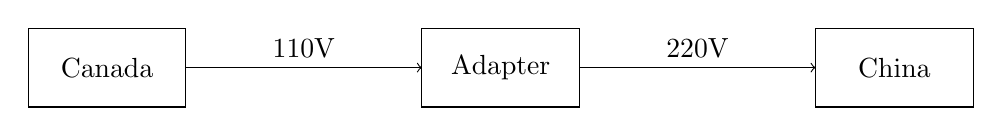
\begin{tikzpicture}
        \draw (0,0) rectangle node{Canada} (2,1);
        \draw (5,0) rectangle node{Adapter} (7,1);
        \draw (10,0) rectangle node{China} (12,1);
        \draw[->] (2,0.5) -- (3.5,0.5)node[above]{110V} -- (5,0.5);
        \draw[->] (7,0.5) -- (8.5,0.5)node[above]{220V} -- (10,0.5);
    \end{tikzpicture}
    \caption{电压转换}
\end{figure}

适配器模式是作为两个不兼容的接口之间的桥梁。这种类型的设计模式属于结构型模式,它结合了两个独立接口的功能,将一个类的接口转换成希望的另外一个接口。适配器模式使得原本由于接口不兼容而不能一起工作的那些类可以一起工作。\\

\mybox{适配器模式}\\

\begin{figure}[H]
    \centering
    \begin{tikzpicture}
        \begin{interface}[text width = 7cm]{ChinaVoltageStandard}{-4,0}
            \operation{+ powerWithChinaStandard() : void}
        \end{interface}

        \begin{class}[text width = 3cm]{ChinaPlug}{-4,3}
            \implement{ChinaVoltageStandard}
        \end{class}

        \begin{interface}[text width = 7cm]{CanadaVoltageStandard}{4,0}
            \operation{+ powerWithChinaStandard() : void}
        \end{interface}

        \begin{class}[text width = 3cm]{CanadaPlug}{4,3}
            \implement{CanadaVoltageStandard}
        \end{class}

        \begin{class}[text width = 8cm]{CanadaAdapter}{-2,7}
            \implement{CanadaVoltageStandard}
            \attribute{- chinaPlug : ChinaPlug}
            \operation{+ CanadaAdapter(ChinaPlug chinaPlug)}
        \end{class}

        \begin{class}[text width = 7cm]{AdapterPatternDemo}{0,11}
            \operation{+ main(String[] args) : void}
        \end{class}

        \draw[umlcd style dashed line, ->] (CanadaAdapter.south) -- (ChinaPlug.north);
        \draw[umlcd style dashed line, ->] (AdapterPatternDemo.south) node[right, black, xshift=-1cm, yshift=-1.5cm]{<<use>>} -- (CanadaAdapter.north);
    \end{tikzpicture}
\end{figure}

\vspace{0.5cm}

\begin{lstlisting}[language=Java, title=ChinaVoltageStandard.java]
public interface ChinaVoltageStandard {
    void powerWithChinaStandard();
}    
\end{lstlisting}

\begin{lstlisting}[language=Java, title=ChinaPlug.java]
public class ChinaPlug implements ChinaVoltageStandard {
    @Override
    public void powerWithChinaStandard() {
        System.out.println("Using China standard (220V)...");
    }
}
\end{lstlisting}

\begin{lstlisting}[language=Java, title=CanadaVoltageStandard.java]
public interface CanadaVoltageStandard {
    void powerWithCanadaStandard();
}
\end{lstlisting}

\begin{lstlisting}[language=Java, title=CanadaPlug.java]
public class CanadaPlug implements CanadaVoltageStandard {
    @Override
    public void powerWithCanadaStandard() {
        System.out.println("Using Canada standard (110V)...");
    }
}
\end{lstlisting}

\begin{lstlisting}[language=Java, title=CanadaAdapter.java]
public class CanadaAdapter implements CanadaVoltageStandard {
    private ChinaPlug chinaPlug;

    public CanadaAdapter(ChinaPlug chinaPlug) {
        this.chinaPlug = chinaPlug;
    }

    @Override
    public void powerWithCanadaStandard() {
        chinaPlug.powerWithChinaStandard();
    }
}
\end{lstlisting}

\begin{lstlisting}[language=Java, title=AdapterPatternDemo.java]
public class AdapterPatternDemo {
    public static void main(String[] args) {
        CanadaPlug canadaPlug = new CanadaPlug();
        canadaPlug.powerWithCanadaStandard();

        ChinaPlug chinaPlug = new ChinaPlug();
        CanadaAdapter adapter = new CanadaAdapter(chinaPlug);
        adapter.powerWithCanadaStandard();
    }
}
\end{lstlisting}

\begin{tcolorbox}
    \mybox{运行结果}
    \begin{verbatim}
Using Canada standard (110V)...
Using China standard (220V)...
\end{verbatim}
\end{tcolorbox}

\newpage

\section{桥接模式}

\subsection{桥接模式(Bridge Pattern)}

桥接模式是一种结构型设计模式, 用于将一个大类或一系列紧密相关的类拆分为抽象和实现两个独立的层次结构, 从而能在开发时分别使用,而降低了抽象和实现这两个可变维度的耦合度。\\

桥接模式通过将继承改为组合的方式来解决这个问题,也就是抽取其中一个维度并使之成为独立的类层次, 这样就可以在初始类中引用这个新层次的对象, 从而使得一个类不必拥有所有的状态和行为。

\begin{figure}[H]
    \centering
    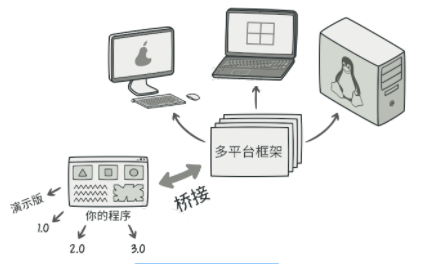
\includegraphics{img/C4/4-8/1.png}
    \caption{跨平台程序}
\end{figure}

\vspace{0.5cm}

\mybox{桥接模式}\\

\begin{figure}[H]
    \centering
    \begin{tikzpicture}
        \begin{class}[text width = 7cm]{BridgePatternDemo}{0,0}
            \operation{+ main(String[] args) : void}
        \end{class}

        \begin{abstractclass}{Program}{-5,6}
            \attribute{- os : OS}
            \operation{+ Program(OS os)}
            \operation{+ getOS() : String}
            \operation{+ programInfo() : void}
        \end{abstractclass}

        \begin{class}{Version}{-5,9}
            \inherit{Program}
            \operation{+ Version(OS os)}
        \end{class}

        \begin{interface}{OS}{4,5}
            \operation{+ getOS() : String}
        \end{interface}

        \begin{class}[text width = 3cm]{Linux}{4,9}
            \implement{OS}
        \end{class}

        \draw[umlcd style dashed line, ->] (Program.east) -- (OS.west);
        \draw[umlcd style dashed line, ->] (BridgePatternDemo.north) node[left, black, xshift=-3cm, yshift=1cm]{<<use>>} -- (Program.south);
        \draw[umlcd style dashed line, ->] (BridgePatternDemo.north) node[right, black, xshift=1.5cm, yshift=1cm]{<<use>>} -- (OS.south);
    \end{tikzpicture}
\end{figure}

\vspace{0.5cm}

\begin{lstlisting}[language=Java, title=OS.java]
public interface OS {
    String getOS();
}
\end{lstlisting}

\begin{lstlisting}[language=Java, title=Linux.java]
public class Linux implements OS {
    @Override
    public String getOS() {
        return "Linux";
    }
}
\end{lstlisting}

\begin{lstlisting}[language=Java, title=Program.java]
public abstract class Program {
    private OS os;

    public Program(OS os) {
        this.os = os;
    }

    public String getOS() {
        return os.getOS();
    }

    public abstract void programInfo();
}
\end{lstlisting}

\begin{lstlisting}[language=Java, title=Version.java]
public class Version extends Program {
    public Version(OS os) {
        super(os);
    }

    @Override
    public void programInfo() {
        System.out.println(
            "Program v1.0 running on " + super.getOS()
        );
    }
}
\end{lstlisting}

\begin{lstlisting}[language=Java, title=BridgePatternDemo.java]
public class BridgePatternDemo {
    public static void main(String[] args) {
        OS os = new Linux();
        Program program = new Version1(os);
        program.programInfo();
    }
}
\end{lstlisting}

\begin{tcolorbox}
    \mybox{运行结果}
    \begin{verbatim}
Program v1.0 running on Linux
\end{verbatim}
\end{tcolorbox}

\newpage

\section{过滤器模式}

\subsection{过滤器模式(Filter Pattern)}

过滤器模式也称标准模式(Criteria Pattern),这种模式允许开发人员使用不同的标准来过滤一组对象,通过逻辑运算以解耦的方式把它们连接起来。过滤器模式属于结构型模式,它结合多个标准来获得单一标准。\\

\mybox{过滤器模式}\\

\begin{figure}[H]
    \centering
    \begin{tikzpicture}
        \begin{interface}[text width = 10cm]{Criteria}{0,0}
            \operation{+ filter(List<Student> students) : List<Student>}
        \end{interface}

        \begin{class}[text width = 3cm]{CriteriaMale}{-8,1}
            \implement{Criteria}
        \end{class}

        \begin{class}[text width = 3cm]{CriteriaCS}{-8,-2}
            \implement{Criteria}
        \end{class}

        \begin{class}[text width = 6cm]{AndCriteria}{-6,5}
            \implement{Criteria}
            \attribute{- criteria1 : Criteria}
            \attribute{- criteria2 : Criteria}
            \operation{+ AndCriteria(Criteria criteria1, Criteria criteria2)}
        \end{class}

        \begin{class}[text width = 6cm]{OrCriteria}{2,5}
            \implement{Criteria}
            \attribute{- criteria1 : Criteria}
            \attribute{- criteria2 : Criteria}
            \operation{+ OrCriteria(Criteria criteria1, Criteria criteria2)}
        \end{class}

        \begin{class}[text width = 6cm]{Student}{-7,-4}
            \attribute{- name : String}
            \attribute{- gender : String}
            \attribute{- major : String}
            \operation{+ Student(String name, String gender, String major)}
            \operation{+ getName() : String}
            \operation{+ getGender() : String}
            \operation{+ getMajor() : String}
        \end{class}

        \begin{class}[text width = 6cm]{FilterPatternDemo}{2,-6}
            \operation{+ main(String[] args) : void}
            \operation{+ printStudents(List<Student> students) : void}
        \end{class}

        \draw[umlcd style dashed line, ->] (FilterPatternDemo.north) node[right, black, xshift=-1cm, yshift=1.75cm]{<<use>>} -- (Criteria.south);
        \draw[umlcd style dashed line, ->] (FilterPatternDemo.west) node[above, black, xshift=-1.5cm, yshift=0.5cm]{<<use>>} -- (Student.east);
    \end{tikzpicture}
\end{figure}

\vspace{0.5cm}

\begin{lstlisting}[language=Java, title=Student.java]
public class Student {
    private String name;
    private String gender;
    private String major;

    public Student(String name, String gender, String major) {
        this.name = name;
        this.gender = gender;
        this.major = major;
    }

    public String getName() {
        return name;
    }

    public String getGender() {
        return gender;
    }

    public String getMajor() {
        return major;
    }
}
\end{lstlisting}

\begin{lstlisting}[language=Java, title=Criteria.java]
import java.util.List;

public interface Criteria {
    List<Student> filter(List<Student> students);
}
\end{lstlisting}

\begin{lstlisting}[language=Java, title=CriteriaMale.java]
import java.util.ArrayList;
import java.util.List;

public class CriteriaMale implements Criteria {
    @Override
    public List<Student> filter(List<Student> students) {
        List<Student> maleStudents = new ArrayList<Student>();
        for(Student student : students) {
            if(student.getGender().equalsIgnoreCase("MALE")) {
                maleStudents.add(student);
            }
        }
        return maleStudents;
    }
}
\end{lstlisting}

\begin{lstlisting}[language=Java, title=CriteriaCS.java]
import java.util.ArrayList;
import java.util.List;

public class CriteriaCS implements Criteria {
    @Override
    public List<Student> filter(List<Student> students) {
        List<Student> csStudents = new ArrayList<Student>();
        for(Student student : students) {
            if(student.getMajor().equalsIgnoreCase("CS")) {
                csStudents.add(student);
            }
        }
        return csStudents;
    }
}
\end{lstlisting}

\begin{lstlisting}[language=Java, title=AndCriteria.java]
import java.util.List;

public class AndCriteria implements Criteria {
    private Criteria criteria1;
    private Criteria criteria2;

    public AndCriteria(Criteria criteria1, Criteria criteria2) {
        this.criteria1 = criteria1;
        this.criteria2 = criteria2;
    }

    @Override
    public List<Student> filter(List<Student> students) {
        return criteria2.filter(criteria1.filter(students));
    }
}
\end{lstlisting}

\begin{lstlisting}[language=Java, title=OrCriteria.java]
import java.util.List;

public class OrCriteria implements Criteria {
    private Criteria criteria1;
    private Criteria criteria2;

    public OrCriteria(Criteria criteria1, Criteria criteria2) {
        this.criteria1 = criteria1;
        this.criteria2 = criteria2;
    }

    @Override
    public List<Student> filter(List<Student> students) {
        List<Student> list1 = criteria1.filter(students);
        List<Student> list2 = criteria2.filter(students);
        list1.removeAll(list2);
        list1.addAll(list2);
        return list1;
    }
}
\end{lstlisting}

\begin{lstlisting}[language=Java, title=FilterPatternDemo.java]
import java.util.ArrayList;
import java.util.Arrays;
import java.util.List;

public class FilterPatternDemo {
    public static void main(String[] args) {
        List<Student> students = new ArrayList<Student>();
        students.add(new Student("Terry", "male", "CS"));
        students.add(new Student("Bob", "male", "Math"));
        students.add(new Student("Anna", "female", "Food Science"));
        students.add(new Student("Lily", "female", "CS"));
        students.add(new Student("Alice", "female", "Art"));

        Criteria male = new CriteriaMale();
        Criteria cs = new CriteriaCS();
        Criteria maleAndCs = new AndCriteria(male, cs);
        Criteria maleOrCs = new OrCriteria(male, cs);

        System.out.println("MALE:");
        printStudents(male.filter(students));

        System.out.println("CS:");
        printStudents(cs.filter(students));

        System.out.println("Male and CS:");
        printStudents(maleAndCs.filter(students));

        System.out.println("Male or CS:");
        printStudents(maleOrCs.filter(students));
    }

    public static void printStudents(List<Student> students) {
        System.out.print("\t");
        for(Student student : students) {
            System.out.print(student.getName() + " ");
        }
        System.out.println();
    }
}  
\end{lstlisting}

\begin{tcolorbox}
    \mybox{运行结果}
    \begin{verbatim}
MALE:
    Terry Bob 
CS:
    Terry Lily 
Male and CS:
    Terry 
Male or CS:
    Bob Terry Lily
\end{verbatim}
\end{tcolorbox}

\newpage

\section{组合模式}

\subsection{组合模式(Composite Pattern)}

在现实生活中,存在很多“整体-部分”的关系,例如,大学的学院与部门、公司的分公司与部门。在软件开发中也是这样,例如,文件夹与文件、容器与控件等。对这些简单对象与复合对象的处理,如果用组合模式来实现会很方便。\\

组合模式属于结构型模式,用于把一组相似的对象当作一个单一的对象,组合模式将对象组合成树形结构以表示“整体-部分”的层次结构。组合模式模糊了简单元素和复杂元素的概念,可以像处理简单元素一样来处理复杂元素,从而使得复杂元素的内部结构解耦。\\

\begin{figure}[H]
    \centering
    \begin{tikzpicture}[
            level distance=2.5cm,
            level 1/.style={sibling distance=6cm},
            level 2/.style={sibling distance=2cm},
            level 3/.style={sibling distance=2cm}
        ]
        \node {技术总监}
        child {
                node {项目经理A}
                child {node {员工A}}
                child {node {员工B}}
                child {node {员工C}}
            }
        child {
                node {项目经理B}
                child {node {员工D}}
                child {node {员工E}}
            };
    \end{tikzpicture}
    \caption{职级关系}
\end{figure}

\vspace{0.5cm}

\mybox{组合模式}\\

\begin{figure}[H]
    \centering
    \begin{tikzpicture}
        \begin{class}[text width = 10cm]{CompositePatternDemo}{0,0}
            \operation{+ main(String[] args) : void}
            \operation{+ indent(int level) : void}
            \operation{+ printEmployeeTree(Employee root, int level) : void}
        \end{class}

        \begin{class}[text width = 9cm]{Employee}{0,9}
            \attribute{- name : String}
            \attribute{- title : String}
            \attribute{- subordinates : List<Employee>}
            \operation{+ Employee(String name, String title)}
            \operation{+ addSubordinate(Employee employee) : void}
            \operation{+ getSubordinates() : List<Employee>}
            \operation{+ toString() : String}
        \end{class}

        \draw[umlcd style dashed line, ->] (CompositePatternDemo.north) node[right, black, yshift=1.5cm]{<<use>>} -- (Employee.south);
    \end{tikzpicture}
\end{figure}

\vspace{0.5cm}

\begin{lstlisting}[language=Java, title=Employee.java]
import java.util.ArrayList;
import java.util.List;

public class Employee {
    private String name;
    private String title;
    private List<Employee> subordinates;

    public Employee(String name, String title) {
        this.name = name;
        this.title = title;
        this.subordinates = new ArrayList<Employee>();
    }

    public void addSubordinate(Employee employee) {
        subordinates.add(employee);
    }

    public List<Employee> getSubordinates() {
        return subordinates;
    }

    @Override
    public String toString() {
        return "Name: " + name + "\t\tTitle: " + title;
    }
}
\end{lstlisting}

\begin{lstlisting}[language=Java, title=CompositePatternDemo.java]
public class CompositePatternDemo {
    public static void main(String[] args) {
        Employee CTO = new Employee("Terry", "CTO");

        Employee pm1 = new Employee("Henry", "Project Manager");
        Employee pm2 = new Employee("Bob", "Project Manager");

        Employee e1 = new Employee("Lily", "Java Engineer");
        Employee e2 = new Employee("Alice", "Python Engineer");
        Employee e3 = new Employee("Eric", "C Engineer");

        pm1.addSubordinate(e1);
        pm1.addSubordinate(e2);
        pm2.addSubordinate(e3);

        CTO.addSubordinate(pm1);
        CTO.addSubordinate(pm2);

        printEmployeeTree(CTO, 0);
    }

    public static void indent(int level) {
        for(int i = 0; i < level; i++) {
            System.out.print("\t");
        }
    }

    public static void printEmployeeTree(Employee root, int level) {
        System.out.println(root);
        for(Employee e : root.getSubordinates()) {
            indent(++level);
            if(!e.getSubordinates().isEmpty()) {
                printEmployeeTree(e, level);
            } else {
                System.out.println(e);
            }
            level--;
        }
    }
}  
\end{lstlisting}

\begin{tcolorbox}
    \mybox{运行结果}
    \begin{verbatim}
Name: Terry		Title: CTO
    Name: Henry		Title: Project Manager
        Name: Lily		Title: Java Engineer
        Name: Alice		Title: Python Engineer
    Name: Bob		Title: Project Manager
        Name: Eric		Title: C Engineer
\end{verbatim}
\end{tcolorbox}

\newpage

\section{装饰器模式}

\subsection{装饰器模式(Decorator Pattern)}

装饰器模式允许向一个现有的对象添加新的功能,同时又不改变其结构装饰器模式属于结构型模式,它用于创建了一个装饰类,用来包装原有的类,并在保持类方法签名完整性的前提下,提供了额外的功能。\\

\mybox{装饰器模式}\\

\begin{figure}[H]
    \centering
    \begin{tikzpicture}
        \begin{interface}{Car}{0,0}
            \operation{+ start() : void}
        \end{interface}

        \begin{class}[text width = 3cm]{Tesla}{-3,2}
            \implement{Car}
        \end{class}

        \begin{class}[text width = 3cm]{Benz}{3,2}
            \implement{Car}
        \end{class}

        \begin{abstractclass}{CarDecorator}{0,-4}
            \implement{Car}
            \attribute{\# car : Car}
            \operation{+ CarDecorator(Car car)}
        \end{abstractclass}

        \begin{class}[text width = 7cm]{AutopilotCarDecorator}{0,-8}
            \inherit{CarDecorator}
            \operation{+ AutopilotCarDecorator(Car car)}
            \operation{+ autopilot() : void}
        \end{class}

        \begin{class}[text width = 7cm]{DecoratorPatternDemo}{0,-12}
            \operation{+ main(String[] args) : void}
        \end{class}

        \draw[umlcd style dashed line, ->] (DecoratorPatternDemo.north) node[right, black, yshift=1cm]{<<use>>} -- (AutopilotCarDecorator.south);
    \end{tikzpicture}
\end{figure}

\vspace{0.5cm}

\begin{lstlisting}[language=Java, title=Car.java]
public interface Car {
    void start();
}
\end{lstlisting}

\begin{lstlisting}[language=Java, title=Tesla.java]
public class Tesla implements Car {
    @Override
    public void start() {
        System.out.println("Tesla start engine...");
    }
}
\end{lstlisting}

\begin{lstlisting}[language=Java, title=Benz.java]
public class Benz implements Car {
    @Override
    public void start() {
        System.out.println("Benz start enginee...");
    }
}
\end{lstlisting}

\begin{lstlisting}[language=Java, title=CarDecorator.java]
public abstract class CarDecorator implements Car {
    protected Car car;

    public CarDecorator(Car car) {
        this.car = car;
    }

    public void start() {
        car.start();
    }
}
\end{lstlisting}

\begin{lstlisting}[language=Java, title=AutopilotCarDecorator.java]
public class AutopilotCarDecorator extends CarDecorator {
    public AutopilotCarDecorator(Car car) {
        super(car);
    }

    public void autopilot() {
        System.out.println("Start autopilot mode...");
    }

    @Override
    public void start() {
        car.start();
        autopilot();
    }
}
\end{lstlisting}

\begin{lstlisting}[language=Java, title=DecoratorPatternDemo.java]
public class DecoratorPatternDemo {
    public static void main(String[] args) {
        Car benz = new Benz();
        benz.start();
        System.out.println("===================");
        Car autopilotTesla = new AutopilotCarDecorator(new Tesla());
        autopilotTesla.start();
    }
}
\end{lstlisting}

\begin{tcolorbox}
    \mybox{运行结果}
    \begin{verbatim}
Benz start enginee...
===================
Tesla start engine...
Start autopilot mode...
\end{verbatim}
\end{tcolorbox}

\newpage

\section{外观模式}

\subsection{外观模式(Facade Pattern)}

外观模式属于结构型模式,它为子系统的众多接口提供了统一的高层接口,使子系统更容易使用。\\

例如KFC有众多基础产品,比如鸡翅、汉堡、薯条、沙拉、可乐等。这些琳琅满目的菜品虽好,但有些顾客犯了选择困难症,不知道该选什么好。于是KFC对这些菜品做了一定的组合,推出了各种各样的套餐。比如A套餐:汉堡+薯条+可乐;B套餐:汉堡+鸡翅+沙拉。\\

\mybox{外观模式}\\

\begin{figure}[H]
    \centering
    \begin{tikzpicture}
        \begin{interface}{Item}{0,0}
            \operation{+ getName() : String}
        \end{interface}

        \begin{class}[text width = 2cm]{Burger}{-6,2}
            \implement{Item}
        \end{class}

        \begin{class}[text width = 2cm]{Fries}{-3,2}
            \implement{Item}
        \end{class}

        \begin{class}[text width = 2cm]{Coke}{0,2}
            \implement{Item}
        \end{class}

        \begin{class}[text width = 2cm]{Chicken}{3,2}
            \implement{Item}
        \end{class}

        \begin{class}[text width = 2cm]{Salad}{6,2}
            \implement{Item}
        \end{class}

        \begin{class}{ComboManager}{-4,-4}
            \attribute{- burger : Item}
            \attribute{- fries : Item}
            \attribute{- coke : Item}
            \attribute{- chicken : Item}
            \attribute{- salad : Item}
            \operation{+ ComboManager()}
            \operation{+ comboA() : void}
            \operation{+ comboB() : void}
        \end{class}

        \begin{class}[text width = 7cm]{FacadePatternDemo}{5,-6}
            \operation{+ main(String[] args) : void}
        \end{class}

        \draw[umlcd style dashed line, ->] (ComboManager.north) -- (Item.south);
        \draw[umlcd style dashed line, ->] (FacadePatternDemo.west) node[above, black, xshift=-1cm]{<<use>>} -- (ComboManager.east);
    \end{tikzpicture}
\end{figure}

\vspace{0.5cm}

\begin{lstlisting}[language=Java, title=Item.java]
public interface Item {
    String getName();
}    
\end{lstlisting}

\begin{lstlisting}[language=Java, title=Burger.java]
public class Burger implements Item {
    @Override
    public String getName() {
        return "Burger";
    }
}
\end{lstlisting}

\begin{lstlisting}[language=Java, title=Fries.java]
public class Fries implements Item {
    @Override
    public String getName() {
        return "Fries";
    }
}
\end{lstlisting}

\begin{lstlisting}[language=Java, title=Coke.java]
public class Coke implements Item {
    @Override
    public String getName() {
        return "Coke";
    }
}
\end{lstlisting}

\begin{lstlisting}[language=Java, title=Chicken.java]
public class Chicken implements Item {
    @Override
    public String getName() {
        return "Chicken";
    }
}
\end{lstlisting}

\begin{lstlisting}[language=Java, title=Salad.java]
public class Salad implements Item {
    @Override
    public String getName() {
        return "Salad";
    }
}
\end{lstlisting}

\begin{lstlisting}[language=Java, title=ComboManager.java]
public class ComboManager {
    private Item burger;
    private Item fries;
    private Item coke;
    private Item chicken;
    private Item salad;

    public ComboManager() {
        burger = new Burger();
        fries = new Fries();
        coke = new Coke();
        chicken = new Chicken();
        salad = new Salad();
    }

    public void comboA() {
        System.out.println("Combo A: "
                            + burger.getName() + ", "
                            + fries.getName() + ", "
                            + coke.getName());
    }

    public void comboB() {
        System.out.println("Combo B: "
                + burger.getName() + ", "
                + chicken.getName() + ", "
                + salad.getName());
    }
}
\end{lstlisting}

\begin{lstlisting}[language=Java, title=FacadePatternDemo.java]
public class FacadePatternDemo {
    public static void main(String[] args) {
        ComboManager comboManager = new ComboManager();
        comboManager.comboA();
        comboManager.comboB();
    }
}
\end{lstlisting}

\begin{tcolorbox}
    \mybox{运行结果}
    \begin{verbatim}
Combo A: Burger, Fries, Coke
Combo B: Burger, Chicken, Salad
\end{verbatim}
\end{tcolorbox}

\newpage

\section{享元模式}

\subsection{享元模式(Flyweight Pattern)}

享元模式主要用于减少创建对象的数量,以减少内存占用和提高性能。享元模式尝试重用现有的同类对象,如果未找到匹配的对象,则创建新对象。享元模式属于结构型模式,它提供了减少对象数量从而改善应用所需的对象结构的方式。\\

\mybox{享元模式}\\

\begin{figure}[H]
    \centering
    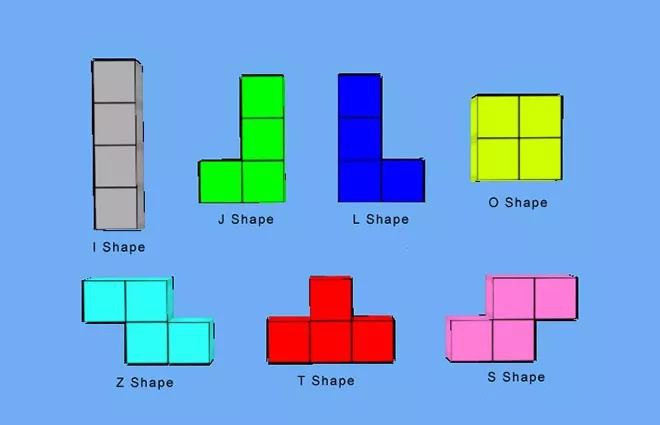
\includegraphics[scale=0.6]{img/C4/4-13/1.png}
    \caption{俄罗斯方块}
\end{figure}

\begin{figure}[H]
    \centering
    \begin{tikzpicture}
        \begin{interface}{Tetris}{0,0}
            \operation{+ display() : void}
        \end{interface}

        \begin{class}[text width = 6cm]{Shape}{4,6}
            \implement{Tetris}
            \attribute{- type : String}
            \attribute{- color : String}
            \operation{+ Shape(String type)}
            \operation{+ setColor(String color) : void}
        \end{class}

        \begin{class}[text width = 8cm]{ShapeFactory}{8,0}
            \attribute{- shapeMap : HashMap<String, Shape>}
            \operation{+ getShape(String type) : Shape}
        \end{class}

        \begin{class}[text width = 7cm]{FlyweightPatternDemo}{8,-5}
            \attribute{- types : String[]}
            \attribute{- colors : String[]}
            \operation{+ main(String[] args) : void}
            \operation{+ getRandomType() : String}
            \operation{+ getRandomColor() : String}
        \end{class}

        \draw[umlcd style dashed line, ->] (ShapeFactory.north) -- (Shape.south);
        \draw[umlcd style dashed line, ->] (FlyweightPatternDemo.north) node[left, black, yshift=1cm]{<<use>>} -- (ShapeFactory.south);
    \end{tikzpicture}
\end{figure}

\vspace{0.5cm}

\begin{lstlisting}[language=Java, title=Tetris.java]
public interface Tetris {
    void display();
}
\end{lstlisting}

\begin{lstlisting}[language=Java, title=Shape.java]
public class Shape implements Tetris {
    private String type;
    private String color;

    public Shape(String type) {
        this.type = type;
    }

    public void setColor(String color) {
        this.color = color;
    }

    @Override
    public void display() {
        System.out.println("Shape: " + type + "\tColor: " + color);
    }
}
\end{lstlisting}

\begin{lstlisting}[language=Java, title=ShapeFactory.java]
import java.util.HashMap;

public class ShapeFactory {
    private static HashMap<String, Shape> shapeMap = new HashMap<>();

    public static Shape getShape(String type) {
        Shape shape = shapeMap.get(type);
        if(shape == null) {
            shape = new Shape(type);
            shapeMap.put(type, shape);
            System.out.println("Shape " + type + " created");
        }
        return shape;
    }
}
\end{lstlisting}

\begin{lstlisting}[language=Java, title=FlyweightPatternDemo.java]
public class FlyweightPatternDemo {
    private static final String[] types = {
            "I", "J", "L",
            "O", "S", "T", "Z"
    };

    private static final String[] colors = {
            "grey", "green", "blue",
            "yellow", "indigo", "red", "pink"
    };

    public static void main(String[] args) {
        for(int i = 0; i < 10; i++) {
            Shape shape = ShapeFactory.getShape(getRandomType());
            shape.setColor(getRandomColor());
            shape.display();
        }
    }

    public static String getRandomType() {
        return types[(int)(Math.random() * types.length)];
    }

    public static String getRandomColor() {
        return colors[(int)(Math.random() * colors.length)];
    }
}
\end{lstlisting}

\begin{tcolorbox}
    \mybox{运行结果}
    \begin{verbatim}
Shape Z created
Shape: Z	Color: red
Shape O created
Shape: O	Color: blue
Shape: O	Color: pink
Shape: Z	Color: green
Shape I created
Shape: I	Color: grey
Shape: I	Color: grey
Shape: Z	Color: green
Shape J created
Shape: J	Color: pink
Shape S created
Shape: S	Color: green
Shape: J	Color: green
\end{verbatim}
\end{tcolorbox}

\newpage

\section{代理模式}

\subsection{代理模式(Proxy Pattern)}

代理模式属于结构型模式,其核心是在被调用方和调用方之间增加一个中介者的角色,也就是代理。\\

在现实生活中,同样需要各种各样的代理人,例如房屋中介、留学中介等。引入代理的意义在于代理专门负责完成专业的事情,如果试图省去代理,只会带来更多的麻烦和成本。\\

\mybox{代理模式}\\

\begin{figure}[H]
    \centering
    \begin{tikzpicture}
        \begin{class}[text width = 7cm]{ProxyPatternDemo}{0,0}
            \operation{+ main(String[] args) : void}
        \end{class}

        \begin{interface}{Login}{-7,0}
            \operation{+ login() : void}
        \end{interface}

        \begin{class}{User}{-7,4}
            \implement{Login}
            \attribute{- username : String}
            \operation{+ User(String username)}
        \end{class}

        \begin{class}{UserProxy}{0,4}
            \implement{Login}
            \attribute{- user : User}
            \operation{+ UserProxy(User user)}
        \end{class}

        \draw[umlcd style dashed line, ->] (ProxyPatternDemo.north) node[left, black, yshift=1cm]{<<use>>} -- (UserProxy.south);
    \end{tikzpicture}
\end{figure}

\vspace{0.5cm}

\begin{lstlisting}[language=Java, title=Login.java]
public interface Login {
    void login();
}
\end{lstlisting}

\begin{lstlisting}[language=Java, title=User.java]
public class User implements Login {
    private String username;

    public User(String username) {
        this.username = username;
    }

    @Override
    public void login() {
        System.out.println(username + " login succeed.");
    }
}
\end{lstlisting}

\begin{lstlisting}[language=Java, title=UserProxy.java]
public class UserProxy implements Login {
    private User user;

    public UserProxy(User user) {
        this.user = user;
    }

    @Override
    public void login() {
        System.out.println("Check username / password...");
        user.login();
    }
}
\end{lstlisting}

\begin{lstlisting}[language=Java, title=ProxyPatternDemo.java]
public class ProxyPatternDemo {
    public static void main(String[] args) {
        Login login = new UserProxy(new User("Admin"));
        login.login();
    }
}
\end{lstlisting}

\begin{tcolorbox}
    \mybox{运行结果}
    \begin{verbatim}
Check username / password...
Admin login succeed.
\end{verbatim}
\end{tcolorbox}

\newpage

\section{责任链模式}

\subsection{责任链模式(Chain of Responsibility Pattern)}

责任链模式属于行为型模式,该模式构造一系列分别担当不同职责的类对象来共同完成一个任务,这些类的对象之间像链条一样紧密相连。如果一个对象不能处理该请求,那么它会把相同的请求传给下一个接收者,依此类推。\\

\mybox{责任链模式}\\

\begin{figure}[H]
    \centering
    \begin{tikzpicture}
        \begin{class}[text width = 8cm]{ChainOfResponsibilityPatternDemo}{0,0}
            \operation{+ main(String[] args) : void}
            \operation{- getLogChain() : Logger}
        \end{class}

        \begin{abstractclass}[text width = 8cm]{Logger}{0,10}
            \attribute{+ INFO : int}
            \attribute{+ DEBUG : int}
            \attribute{+ ERROR : int}
            \attribute{\# level : int}
            \attribute{\# nextLogger : Logger}
            \operation{+ setNextLogger(Logger nextLogger) : void}
            \operation{\# write(String msg) : void}
            \operation{+ login(int level, String msg) : void}
        \end{abstractclass}

        \begin{class}{ConsoleLogger}{-8,10}
            \inherit{Logger}
            \operation{+ ConsoleLogger(int level)}
        \end{class}

        \begin{class}{FileLogger}{-8,7}
            \inherit{Logger}
            \operation{+ FileLogger(int level)}
        \end{class}

        \begin{class}{ErrorLogger}{-8,4}
            \inherit{Logger}
            \operation{+ ErrorLogger(int level)}
        \end{class}

        \draw[umlcd style dashed line, ->] (ChainOfResponsibilityPatternDemo.north) node[left, black, yshift=1cm]{<<use>>} -- (Logger.south);
    \end{tikzpicture}
\end{figure}

\vspace{0.5cm}

\begin{lstlisting}[language=Java, title=Logger.java]
public abstract class Logger {
    public static int INFO = 1;
    public static int DEBUG = 2;
    public static int ERROR = 3;

    protected int level;
    protected Logger nextLogger;

    public void setNextLogger(Logger nextLogger) {
        this.nextLogger = nextLogger;
    }

    protected abstract void write(String msg);

    public void log(int level, String msg) {
        if(this.level <= level) {
            write(msg);
        }
        if(nextLogger != null) {
            nextLogger.log(level, msg);
        }
    }
}
\end{lstlisting}

\begin{lstlisting}[language=Java, title=ConsoleLogger.java]
public class ConsoleLogger extends Logger {
    public ConsoleLogger(int level) {
        this.level = level;
    }

    @Override
    protected void write(String msg) {
        System.out.println("Console: " + msg);
    }
}
\end{lstlisting}

\begin{lstlisting}[language=Java, title=FileLogger.java]
public class FileLogger extends Logger {
    public FileLogger(int level) {
        this.level = level;
    }

    @Override
    protected void write(String msg) {
        System.out.println("File: " + msg);
    }
}
\end{lstlisting}

\begin{lstlisting}[language=Java, title=ErrorLogger.java]
public class ErrorLogger extends Logger {
    public ErrorLogger(int level) {
        this.level = level;
    }

    @Override
    protected void write(String msg) {
        System.out.println("Error: " + msg);
    }
}
\end{lstlisting}

\begin{lstlisting}[language=Java, title=ChainOfResponsibilityPatternDemo.java]
public class ChainOfResponsibilityPatternDemo {
    public static void main(String[] args) {
        Logger logChain = getLogChain();

        logChain.log(Logger.INFO, "[INFO] Hello world!");
        logChain.log(Logger.DEBUG, "[DEBUG] Hello world!");
        logChain.log(Logger.ERROR, "[ERROR] Hello world!");
    }

    private static Logger getLogChain() {
        Logger errorLogger = new ErrorLogger(Logger.ERROR);
        Logger fileLogger = new FileLogger(Logger.DEBUG);
        Logger consoleLogger = new ConsoleLogger(Logger.INFO);

        errorLogger.setNextLogger(fileLogger);
        fileLogger.setNextLogger(consoleLogger);
        return errorLogger;
    }
}
\end{lstlisting}

\begin{tcolorbox}
    \mybox{运行结果}
    \begin{verbatim}
Console: [INFO] Hello world!
File: [DEBUG] Hello world!
Console: [DEBUG] Hello world!
Error: [ERROR] Hello world!
File: [ERROR] Hello world!
Console: [ERROR] Hello world!
\end{verbatim}
\end{tcolorbox}

\newpage

\section{命令模式}

\subsection{命令模式(Command Pattern)}

命令模式属于行为型模式,请求以命令的形式包裹在对象中,并传给调用对象。调用对象寻找可以处理该命令的合适的对象,并把该命令传给相应的对象,该对象执行命令。\\

在软件系统中,行为请求者与行为实现者通常是一种紧耦合的关系,但某些场合,比如需要对行为进行记录、撤销或重做、事务等处理时,这种无法抵御变化的紧耦合的设计就不太合适。\\

\mybox{命令模式}\\

\begin{figure}[H]
    \centering
    \begin{tikzpicture}
        \begin{interface}{Order}{0,0}
            \operation{+ execute() : void}
        \end{interface}

        \begin{class}[text width = 6cm]{PurchaseOrder}{8,0}
            \implement{Order}
            \attribute{- dish : Dish}
            \operation{+ PurchaseOrder(Dish dish)}
        \end{class}

        \begin{class}[text width = 9cm]{Dish}{4,6}
            \attribute{- name : String}
            \attribute{- price : double}
            \attribute{- quantity : int}
            \operation{+ Dish(String name, double price, int quantity)}
            \operation{+ purchase() : void}
        \end{class}

        \begin{class}[text width = 6cm]{OrderSystem}{0,-4}
            \attribute{- orderList : List<Order>}
            \operation{+ takeOrder(Order order) : void}
            \operation{+ handleOrders() : void}
        \end{class}

        \begin{class}[text width = 7cm]{CommandPatternDemo}{9,-5}
            \operation{+ main(String[] args) : void}
        \end{class}

        \draw[umlcd style dashed line, ->] (PurchaseOrder.north) -- (Dish.south);
        \draw[umlcd style dashed line, ->] (OrderSystem.north) -- (Order.south);
        \draw[umlcd style dashed line, ->] (CommandPatternDemo.west) node[below, black, xshift=-1cm]{<<use>>} -- (OrderSystem.east);
    \end{tikzpicture}
\end{figure}

\vspace{0.5cm}

\begin{lstlisting}[language=Java, title=Order.java]
public interface Order {
    void execute();
}
\end{lstlisting}

\begin{lstlisting}[language=Java, title=Dish.java]
public class Dish {
    private String name;
    private double price;
    private int quantity;

    public Dish(String name, double price, int quantity) {
        this.name = name;
        this.price = price;
        this.quantity = quantity;
    }

    public void purchase() {
        System.out.println(
            String.format("[%s]\t$%.2f\t*%d", name, price, quantity)
        );
    }
}
\end{lstlisting}

\begin{lstlisting}[language=Java, title=PurchaseOrder.java]
public class PurchaseOrder implements Order {
    private Dish dish;

    public PurchaseOrder(Dish dish) {
        this.dish = dish;
    }

    @Override
    public void execute() {
        dish.purchase();
    }
}
\end{lstlisting}

\begin{lstlisting}[language=Java, title=OrderSystem.java]
import java.util.ArrayList;
import java.util.List;

public class OrderSystem {
    private List<Order> orderList = new ArrayList<>();

    public void takeOrder(Order order) {
        orderList.add(order);
    }

    public void handleOrders() {
        for(Order order : orderList) {
            order.execute();
        }
        orderList.clear();
    }
}
\end{lstlisting}

\begin{lstlisting}[language=Java, title=CommandPatternDemo.java]
public class CommandPatternDemo {
    public static void main(String[] args) {
        PurchaseOrder purchaseOrder1 = new BuyOrder(
            new Dish("Boiled Fish", 20, 1)
        );
        PurchaseOrder purchaseOrder2 = new BuyOrder(
            new Dish("B.B.Q Pork", 15, 2)
        );
        PurchaseOrder purchaseOrder3 = new BuyOrder(
            new Dish("Lemon beef", 25, 1)
        );

        OrderSystem orderSystem = new OrderSystem();
        orderSystem.takeOrder(purchaseOrder1);
        orderSystem.takeOrder(purchaseOrder2);
        orderSystem.takeOrder(purchaseOrder3);

        orderSystem.handleOrders();
    }
}
\end{lstlisting}

\begin{tcolorbox}
    \mybox{运行结果}
    \begin{verbatim}
[Boiled Fish]	$20.00	*1
[B.B.Q Pork]	$15.00	*2
[Lemon beef]	$25.00	*1
\end{verbatim}
\end{tcolorbox}

\newpage

\section{解释器模式}

\subsection{解释器模式(Interpreter Pattern)}

在编译原理中,一个算术表达式通过词法分析器形成词法单元,而后这些词法单元再通过语法分析器构建语法分析树,最终形成一个抽象语法分析树。\\

如果一种特定类型的问题发生的频率足够高,那么可能就值得将该问题的各个实例表述为一个简单语言中的句子,这样就可以构建一个解释器,该解释器通过解释这些句子来解决该问题。比如正则表达式就是解释器模型的一种应用,解释器为正则表达式定义了一个文法、如何表示一个特定的正则表达式、以及如何解释这个正则表达式。\\

解释器模式属于行为型模式,提供了评估语言的语法或表达式的方式,这种模式实现了一个表达式接口,该接口解释一个特定的上下文。解释器模式常被用于SQL解析、符号处理引擎等领域。\\

\mybox{解释器模式}\\

\begin{figure}[H]
    \centering
    \begin{tikzpicture}
        \begin{interface}{Expression}{0,0}
            \operation{+ interprete() : int}
        \end{interface}

        \begin{class}{Number}{-6,4}
            \implement{Expression}
            \attribute{- num : int}
            \operation{+ Number(int num)}
        \end{class}

        \begin{class}[text width = 9cm]{Addition}{2,4}
            \implement{Expression}
            \attribute{- exp1 : Expression}
            \attribute{- exp2 : Expression}
            \operation{+ Addition(Expression exp1, Expression exp2)}
        \end{class}

        \begin{class}{Calculator}{0,-4}
            \attribute{- stack : Stack<Expression>}
            \operation{+ Calculator(String expression)}
            \operation{+ calculate() : int}
        \end{class}

        \begin{class}[text width = 7cm]{InterpreterPatternDemo}{0,-10}
            \operation{+ main(String[] args) : void}
        \end{class}

        \draw[umlcd style dashed line, ->] (Calculator.north) -- (Expression.south);
        \draw[umlcd style dashed line, ->] (InterpreterPatternDemo.north) node[right, black, yshift=1cm]{<<use>>} -- (Calculator.south);
    \end{tikzpicture}
\end{figure}

\vspace{0.5cm}

\begin{lstlisting}[language=Java, title=Expression.java]
public interface Expression {
    int interpret();
}
\end{lstlisting}

\begin{lstlisting}[language=Java, title=Number.java]
public class Number implements Expression {
    private int num;

    public Number(int num) {
        this.num = num;
    }

    @Override
    public int interpret() {
        return num;
    }
}
\end{lstlisting}

\begin{lstlisting}[language=Java, title=Addition.java]
public class Addition implements Expression {
    private Expression exp1;
    private Expression exp2;

    public Addition(Expression exp1, Expression exp2) {
        this.exp1 = exp1;
        this.exp2 = exp2;
    }

    @Override
    public int interpret() {
        return exp1.interpret() + exp2.interpret();
    }
}
\end{lstlisting}

\begin{lstlisting}[language=Java, title=Calculator.java]
import java.util.Stack;

public class Calculator {
    private Stack<Expression> stack = new Stack<>();

    public Calculator(String expression) {
        Expression exp1, exp2;

        String[] elements = expression.split(" ");
        for (int i = 0; i < elements.length; i++) {
            if (elements[i].charAt(0) == '+') {
                exp1 = stack.pop();
                exp2 = new Number(Integer.valueOf(elements[++i]));
                stack.push(new Addition(exp1, exp2));
            } else {
                stack.push(new Number(Integer.valueOf(elements[i])));
            }
        }
    }

    public int calculate() {
        return stack.pop().interpret();
    }
}
\end{lstlisting}

\begin{lstlisting}[language=Java, title=InterpreterPatternDemo.java]
public class InterpreterPatternDemo {
    public static void main(String[] args) {
        Calculator calculator = new Calculator("1 + 22 + 333");
        System.out.println(calculator.calculate());
    }
}  
\end{lstlisting}

\begin{tcolorbox}
    \mybox{运行结果}
    \begin{verbatim}
356
\end{verbatim}
\end{tcolorbox}

\newpage

\section{迭代器模式}

\subsection{迭代器模式(Iterator Pattern)}

迭代器模式属于行为型模式,提供了一种方法顺序访问一个聚合对象中的各种元素,而又不暴露该对象的内部表示。\\

\mybox{迭代器模式}\\

\begin{figure}[H]
    \centering
    \begin{tikzpicture}
        \begin{interface}{Iterator}{0,0}
            \operation{+ hasNext() : boolean}
            \operation{+ next() : Object}
        \end{interface}

        \begin{package}{ArrayIterator}
            \begin{class}{ArrayIterator}{0,5}
                \implement{Iterator}
            \end{class}

            \begin{class}[text width = 6cm]{ArrayContainer}{8,5}
                \attribute{- data : Object[]}
                \operation{+ ArrayContainer(Object[] data)}
                \operation{+ getIterator() : Iterator}
            \end{class}
        \end{package}

        \begin{class}[text width = 7cm]{IteratorPatternDemo}{8,0}
            \operation{+ main(String[] args) : void}
        \end{class}

        \draw[umlcd style dashed line, ->] (IteratorPatternDemo.north) node[right, black, yshift=1cm]{<<use>>} -- (ArrayContainer.south);
    \end{tikzpicture}
\end{figure}

\vspace{0.5cm}

\begin{lstlisting}[language=Java, title=Iterator.java]
public interface Iterator {
    boolean hasNext();
    Object next();
}
\end{lstlisting}

\begin{lstlisting}[language=Java, title=ArrayContainer.java]
public class ArrayContainer {
    private Object[] data;

    private class ArrayIterator implements Iterator {
        private int index;

        @Override
        public boolean hasNext() {
            return index < data.length;
        }

        @Override
        public Object next() {
            if(this.hasNext()) {
                return data[index++];
            }
            return null;
        }
    }

    public ArrayContainer(Object[] data) {
        this.data = data;
    }

    public Iterator getIterator() {
        return new ArrayIterator();
    }
}
\end{lstlisting}

\begin{lstlisting}[language=Java, title=IteratorPatternDemo.java]
public class IteratorPatternDemo {
    public static void main(String[] args) {
        String[] data = {"data1", "data2", "data3", "data4"};
        ArrayContainer arrayContainer = new ArrayContainer(data);
        Iterator iter = arrayContainer.getIterator();
        while(iter.hasNext()) {
            System.out.println(iter.next());
        }
    }
}
\end{lstlisting}

\begin{tcolorbox}
    \mybox{运行结果}
    \begin{verbatim}
data1
data2
data3
data4
\end{verbatim}
\end{tcolorbox}

\newpage

\section{中介者模式}

\subsection{中介者模式(Mediator Pattern)}

中介者模式属于行为型模式,用来降低多个对象和类之间的通信复杂性。中介者模式提供了一个中介类,该类通常处理不同类之间的通信,并支持松耦合,使代码易于维护。\\

\mybox{中介者模式}\\

\begin{figure}[H]
    \centering
    \begin{tikzpicture}
        \begin{class}[text width = 7cm]{MediatorPatternDemo}{0,0}
            \operation{+ main(String[] args) : void}
        \end{class}

        \begin{class}{User}{5,7}
            \attribute{- name : String}
            \operation{+ User(String name)}
            \operation{+ getName() : String}
            \operation{+ sendMessage(String msg) : void}
        \end{class}

        \begin{class}{ChatRoom}{-5,6}
            \operation{+ showMessage(User user, String msg) : void}
        \end{class}

        \draw[umlcd style dashed line, <->] (ChatRoom.east) -- (User.west);
        \draw[umlcd style dashed line, ->] (MediatorPatternDemo.north) node[right, black, yshift=1cm]{<<use>>} -- (User.south);
    \end{tikzpicture}
\end{figure}

\vspace{0.5cm}

\begin{lstlisting}[language=Java, title=ChatRoom.java]
import java.util.Date;

public class ChatRoom {
    public static void showMessage(User user, String msg) {
        System.out.println(
                String.format("[%s] %s: %s",
                            new Date().toString(),
                            user.getName(),
                            msg)
        );
    }
}
\end{lstlisting}

\begin{lstlisting}[language=Java, title=User.java]
public class User {
    private String name;

    public User(String name) {
        this.name = name;
    }

    public String getName() {
        return name;
    }

    public void sendMessage(String msg) {
        ChatRoom.showMessage(this, msg);
    }
}
\end{lstlisting}

\begin{lstlisting}[language=Java, title=MediatorPatternDemo.java]
public class MediatorPatternDemo {
    public static void main(String[] args) {
        User user1 = new User("Terry");
        User user2 = new User("Lily");

        user1.sendMessage("Hi, Lily!");
        user2.sendMessage("Hello, Terry!");
    }
}
\end{lstlisting}

\begin{tcolorbox}
    \mybox{运行结果}
    \begin{verbatim}
[Wed Dec 01 17:54:29 CST 2021] Terry: Hi, Lily!
[Wed Dec 01 17:54:29 CST 2021] Lily: Hello, Terry!
\end{verbatim}
\end{tcolorbox}

\newpage

\section{备忘录模式}

\subsection{备忘录模式(Memento Pattern)}

备忘录模式属于行为型模式,允许在不暴露对象实现细节的情况下保存和恢复对象之前的状态。\\

例如一款文字编辑器,除了简单的文字编辑功能外,编辑器中还要有让用户能撤销施加在文本上的任何操作,给用户提供了一种可以恢复状态的机制,可以使用户能够比较方便地回到某个历史的状态。 程序在执行任何操作前会记录所有的对象状态,并将其保存下来。当用户此后需要撤销某个操作时,程序将从历史记录中获取最近的快照,然后使用它来恢复所有对象的状态。

\begin{figure}[H]
    \centering
    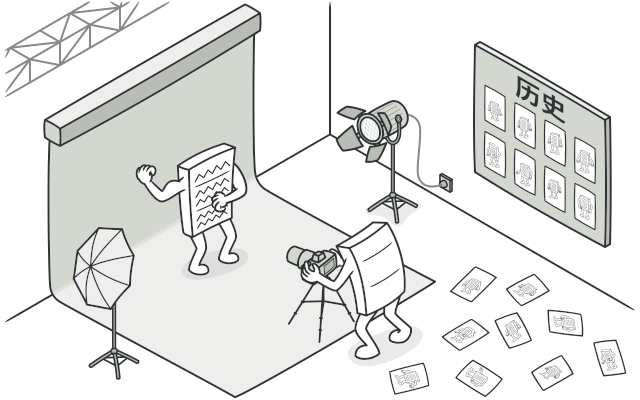
\includegraphics[scale=0.6]{img/C4/4-20/1.png}
    \caption{快照}
\end{figure}

\vspace{0.5cm}

\mybox{备忘录模式}\\

\begin{figure}[H]
    \centering
    \begin{tikzpicture}
        \begin{class}{Memento}{-4,16}
            \attribute{- state : String}
            \operation{+ Memento(String state)}
            \operation{+ getState() : String}
        \end{class}

        \begin{class}[text width = 10cm]{Originator}{4,12}
            \attribute{- state : String}
            \operation{+ setState(String state) : void}
            \operation{+ getState() : String}
            \operation{+ saveStateToMemento() : Memento}
            \operation{+ getStateFromMemento(Memento memento) : void}
        \end{class}

        \begin{class}[text width = 7cm]{CareTaker}{-3,5}
            \attribute{- mementoList : List<Memento>}
            \operation{+ add(Memento memento) : void}
            \operation{+ get(int index) : Memento}
        \end{class}

        \begin{class}[text width = 7cm]{MementoPatternDemo}{0,0}
            \operation{+ main(String[] args) : void}
        \end{class}

        \draw[umlcd style dashed line, ->] (Originator.north) -- (Memento.east);
        \draw[umlcd style dashed line, ->] (CareTaker.north) -- (Memento.south);
        \draw[umlcd style dashed line, ->] (MementoPatternDemo.north) node[right, black, xshift=1.5cm, yshift=3cm]{<<use>>} -- (Originator.south);
        \draw[umlcd style dashed line, ->] (MementoPatternDemo.north) node[left, black, xshift=-0.5cm, yshift=1.5cm]{<<use>>} -- (CareTaker.south);
    \end{tikzpicture}
\end{figure}

\vspace{0.5cm}

\begin{lstlisting}[language=Java, title=Memento.java]
public class Memento {
    private String state;

    public Memento(String state) {
        this.state = state;
    }

    public String getState() {
        return state;
    }
}
\end{lstlisting}

\begin{lstlisting}[language=Java, title=Originator.java]
public class Originator {
    private String state;

    public void setState(String state) {
        this.state = state;
    }

    public String getState() {
        return state;
    }

    public Memento saveStateToMemento() {
        return new Memento(state);
    }

    public void getStateFromMemento(Memento memento) {
        state = memento.getState();
    }
}
\end{lstlisting}

\begin{lstlisting}[language=Java, title=CareTaker.java]
import java.util.ArrayList;
import java.util.List;

public class CareTaker {
    private List<Memento> mementoList = new ArrayList<>();

    public void add(Memento memento) {
        mementoList.add(memento);
    }

    public Memento get(int index) {
        return mementoList.get(index);
    }
}
\end{lstlisting}

\begin{lstlisting}[language=Java, title=MementoPatternDemo.java]
public class MementoPatternDemo {
    public static void main(String[] args) {
        CareTaker careTaker = new CareTaker();
        Originator originator = new Originator();

        originator.setState("State 1");
        originator.setState("State 2");
        careTaker.add(originator.saveStateToMemento());

        originator.setState("State 3");
        careTaker.add(originator.saveStateToMemento());

        originator.setState("State 4");
        System.out.println(
            "Current State: " + originator.getState()
        );

        originator.getStateFromMemento(careTaker.get(0));
        System.out.println(
            "First saved state: " + originator.getState()
        );

        originator.getStateFromMemento(careTaker.get(1));
        System.out.println(
            "Second saved state: " + originator.getState()
        );
    }
}
\end{lstlisting}

\begin{tcolorbox}
    \mybox{运行结果}
    \begin{verbatim}
Current State: State 4
First saved state: State 2
Second saved state: State 3
\end{verbatim}
\end{tcolorbox}

\newpage

\section{观察者模式}

\subsection{观察者模式(Observer Pattern)}

观察者模式属于行为型模式,是一种基于事件和响应的设计模式,常用于窗体应用程序和游戏开发。对象间存在一对多的依赖关系,当一个对象的状态发生改变,所有依赖于它的对象都得到通知并被自动更新。观察者模式主要解决一个对象状态改变给其它对象通知的问题,而且要考虑到易用和低耦合,保证高度的协作。\\

\mybox{观察者模式}\\

\begin{figure}[H]
    \centering
    \begin{tikzpicture}
        \begin{abstractclass}{Observer}{0,0}
            \attribute{\# decimal : Decimal}
            \operation{+ update() : void}
        \end{abstractclass}

        \begin{class}{Binary}{-5,3}
            \inherit{Observer}
            \operation{+ Binary(Decimal decimal)}
        \end{class}

        \begin{class}{Octal}{0,5}
            \inherit{Observer}
            \operation{+ Octal(Decimal decimal)}
        \end{class}

        \begin{class}{Hex}{5,3}
            \inherit{Observer}
            \operation{+ Hex(Decimal decimal)}
        \end{class}

        \begin{class}[text width = 7cm]{Decimal}{-4,-4}
            \attribute{- observers : List<Observer>}
            \attribute{- value : int}
            \operation{+ getValue() : int}
            \operation{+ setValue(int value) : void}
            \operation{+ attach(Observer observer) : void}
            \operation{+ updateAllObservers() : void}
        \end{class}

        \begin{class}[text width = 7cm]{ObserverPatternDemo}{4,-8}
            \operation{+ main(String[] args) : void}
        \end{class}

        \draw[umlcd style dashed line, <->] (Decimal.north) -- (Observer.south);
        \draw[umlcd style dashed line, ->] (ObserverPatternDemo.west) node[right, black, yshift=1.5cm]{<<use>>} -- (Decimal.east);
    \end{tikzpicture}
\end{figure}

\vspace{0.5cm}

\begin{lstlisting}[language=Java, title=Decimal.java]
import java.util.ArrayList;
import java.util.List;

public class Decimal {
    private List<Observer> observers = new ArrayList<>();
    private int value;

    public int getValue() {
        return value;
    }

    public void setValue(int value) {
        this.value = value;
        updateAllObservers();
    }

    public void attach(Observer observer){
        observers.add(observer);
    }

    public void updateAllObservers(){
        for(Observer observer : observers) {
            observer.update();
        }
    }
}
\end{lstlisting}

\begin{lstlisting}[language=Java, title=Observer.java]
public abstract class Observer {
    protected Decimal decimal;
    public abstract void update();
}
\end{lstlisting}

\begin{lstlisting}[language=Java, title=Binary.java]
public class Binary extends Observer {
    public Binary(Decimal decimal) {
        this.decimal = decimal;
        this.decimal.attach(this);
    }

    @Override
    public void update() {
        System.out.println(
            "Binary: " +
            Integer.toBinaryString(decimal.getValue())
        );
    }
}
\end{lstlisting}

\begin{lstlisting}[language=Java, title=Octal.java]
public class Octal extends Observer {
    public Octal(Decimal decimal) {
        this.decimal = decimal;
        this.decimal.attach(this);
    }

    @Override
    public void update() {
        System.out.println(
            "Octal: " +
            Integer.toOctalString(decimal.getValue())
        );
    }
}
\end{lstlisting}

\begin{lstlisting}[language=Java, title=Hex.java]
public class Hex extends Observer {
    public Hex(Decimal decimal) {
        this.decimal = decimal;
        this.decimal.attach(this);
    }

    @Override
    public void update() {
        System.out.println(
            "Hex: " +
            Integer.toHexString(decimal.getValue())
        );
    }
}
\end{lstlisting}

\begin{lstlisting}[language=Java, title=ObserverPatternDemo.java]
public class ObserverPatternDemo {
    public static void main(String[] args) {
        Decimal decimal = new Decimal();
        new Binary(decimal);
        new Octal(decimal);
        new Hex(decimal);

        decimal.setValue(10);
        decimal.setValue(20);
    }
}
\end{lstlisting}

\begin{tcolorbox}
    \mybox{运行结果}
    \begin{verbatim}
Binary: 1010
Octal: 12
Hex: a
Binary: 10100
Octal: 24
Hex: 14
\end{verbatim}
\end{tcolorbox}

\newpage

\section{状态模式}

\subsection{状态模式(State Pattern)}

状态模式属于行为型模式,在状态模式中,允许一个对象在其内部状态改变时改变它的行为,类的行为是基于它的状态改变的。\\

\mybox{状态模式}\\

\begin{figure}[H]
    \centering
    \begin{tikzpicture}
        \begin{interface}{State}{0,8}
            \operation{+ action() : void}
        \end{interface}

        \begin{class}[text width = 3cm]{StartState}{-4,4}
            \implement{State}
        \end{class}

        \begin{class}[text width = 3cm]{StopState}{0,4}
            \implement{State}
        \end{class}

        \begin{class}[text width = 6cm]{Context}{6,5}
            \attribute{- state : State}
            \operation{+ Context()}
            \operation{+ getState() : State}
            \operation{+ setState(State state) : void}
        \end{class}

        \begin{class}[text width = 7cm]{StatePatternDemo}{0,0}
            \operation{+ main(String[] args) : void}
        \end{class}

        \draw[umlcd style dashed line, ->] (Context.north) node[right, black, xshift=-2cm, yshift=1.5cm]{<<use>>} -- (State.east);
        \draw[umlcd style dashed line, ->] (StatePatternDemo.north) node[left, black, xshift=-2.5cm, yshift=1.5cm]{<<use>>} -- (StartState.south);
        \draw[umlcd style dashed line, ->] (StatePatternDemo.north) node[right, black, yshift=1.5cm]{<<use>>} -- (StopState.south);
        \draw[umlcd style dashed line, ->] (StatePatternDemo.north) node[right, black, xshift=2cm, yshift=1cm]{<<use>>} -- (Context.south);
    \end{tikzpicture}
\end{figure}

\vspace{0.5cm}

\begin{lstlisting}[language=Java, title=State.java]
public interface State {
    void action(Context context);
}
\end{lstlisting}

\begin{lstlisting}[language=Java, title=Context.java]
public class Context {
    private State state;

    public Context() {
        state = null;
    }

    public void setState(State state) {
        this.state = state;
    }

    public State getState() {
        return state;
    }
}
\end{lstlisting}

\begin{lstlisting}[language=Java, title=StartState.java]
public class StartState implements State {
    @Override
    public void action(Context context) {
        context.setState(this);
        System.out.println("In start state ...");
    }

    @Override
    public String toString() {
        return "StartState";
    }
}
\end{lstlisting}

\begin{lstlisting}[language=Java, title=StopState.java]
public class StopState implements State {
    @Override
    public void action(Context context) {
        context.setState(this);
        System.out.println("In stop state ...");
    }

    @Override
    public String toString() {
        return "StopState";
    }
}
\end{lstlisting}

\begin{lstlisting}[language=Java, title=StatePatternDemo.java]
public class StatePatternDemo {
    public static void main(String[] args) {
        Context context = new Context();

        StartState startState = new StartState();
        startState.action(context);
        System.out.println(context.getState());

        StopState stopState = new StopState();
        stopState.action(context);
        System.out.println(context.getState());
    }
}
\end{lstlisting}

\begin{tcolorbox}
    \mybox{运行结果}
    \begin{verbatim}
In start state ...
StartState
In stop state ...
StopState
\end{verbatim}
\end{tcolorbox}

\newpage

\section{空对象模式}

\subsection{Null Object Pattern}

平时开发中应该避免过多的判空检查,空对象模式很好地避免了这种情况出现。在空对象模式中,当为空或者不存在的时候返回一个空对象,避免发生程序NullPointException异常。这样的空对象也可以在数据不可用的时候提供默认的行为。\\

\mybox{空对象模式}\\

\begin{figure}[H]
    \centering
    \begin{tikzpicture}
        \begin{abstractclass}{User}{0,9}
            \attribute{\# name : String}
            \operation{+ isNil() : boolean}
            \operation{+ getName() : String}
        \end{abstractclass}

        \begin{class}{RealUser}{-3,12}
            \inherit{User}
            \operation{+ RealUser(String name)}
        \end{class}

        \begin{class}{NullUser}{3,12}
            \inherit{User}
        \end{class}

        \begin{class}{UserFactory}{0,4}
            \operation{+ getUser() : User}
        \end{class}

        \begin{class}[text width = 7cm]{NullObjectPatternDemo}{0,0}
            \operation{+ main(String[] args) : void}
        \end{class}

        \draw[umlcd style dashed line, ->] (UserFactory.north) node[right, black, yshift=0.5cm]{<<create>>} -- (User.south);
        \draw[umlcd style dashed line, ->] (NullObjectPatternDemo.north) node[right, black, yshift=1cm]{<<use>>} -- (UserFactory.south);
    \end{tikzpicture}
\end{figure}

\vspace{0.5cm}

\begin{lstlisting}[language=Java, title=User.java]
public abstract class User {
    protected String name;

    public abstract boolean isNil();

    public abstract String getName();
}
\end{lstlisting}

\begin{lstlisting}[language=Java, title=RealUser.java]
public class RealUser extends User {
    public RealUser(String name) {
        this.name = name;
    }

    @Override
    public boolean isNil() {
        return false;
    }

    @Override
    public String getName() {
        return name;
    }
}
\end{lstlisting}

\begin{lstlisting}[language=Java, title=NullUser.java]
public class NullUser extends User {
    @Override
    public boolean isNil() {
        return true;
    }

    @Override
    public String getName() {
        return "N/A";
    }
}
\end{lstlisting}

\begin{lstlisting}[language=Java, title=UserFactory.java]
public class UserFactory {
    public static final String[] names = {
        "Terry", "Lily", "Henry", "Bob"
    };

    public static User getUser(String name) {
        for(int i = 0; i < names.length; i++) {
            if(names[i].equalsIgnoreCase(name)) {
                return new RealUser(name);
            }
        }
        return new NullUser();
    }
}
\end{lstlisting}

\begin{lstlisting}[language=Java, title=NullObjectPatternDemo.java]
public class NullObjectPatternDemo {
    public static void main(String[] args) {
        User user1 = UserFactory.getUser("Terry");
        User user2 = UserFactory.getUser("John");
        User user3 = UserFactory.getUser("Alice");
        User user4 = UserFactory.getUser("Lily");

        System.out.println(user1.getName());
        System.out.println(user2.getName());
        System.out.println(user3.getName());
        System.out.println(user4.getName());
    }
}
\end{lstlisting}

\begin{tcolorbox}
    \mybox{运行结果}
    \begin{verbatim}
Terry
N/A
N/A
Lily
\end{verbatim}
\end{tcolorbox}

\newpage

\section{策略模式}

\subsection{策略模式(Strategy Pattern)}

策略模式属于行为型模式,在策略模式中一个类的行为或其算法可以在运行时更改。策略指的是可以实现目标的方案集合,在某些特定情况下,策略之间是可以相互替换的。\\

策略模式将每一个算法封装起来,并让它们可以相互替换。策略模式只适用管理一组同类型的算法,并且这些算法是完全互斥的情况,也就是说任何时候,多个策略中只有一个可以生效。\\

\mybox{策略模式}\\

\begin{figure}[H]
    \centering
    \begin{tikzpicture}
        \begin{interface}[text width = 7cm]{Strategy}{0,10}
            \operation{+ calculate(int num1, int num2) : int}
        \end{interface}

        \begin{class}[text width = 3cm]{Addition}{-4,4}
            \implement{Strategy}
        \end{class}

        \begin{class}[text width = 3cm]{Subtraction}{0,5}
            \implement{Strategy}
        \end{class}

        \begin{class}[text width = 3cm]{Multiplication}{4,4}
            \implement{Strategy}
        \end{class}

        \begin{class}[text width = 6cm]{Context}{8,2}
            \attribute{- strategy : Strategy}
            \operation{+ Context(Strategy strategy)}
            \operation{+ execute(int num1, num2) : int}
        \end{class}

        \begin{class}[text width = 7cm]{StrategyPatternDemo}{0,0}
            \operation{+ main(String[] args) : void}
        \end{class}

        \draw[umlcd style dashed line, ->] (Context.north) node[right, black, xshift=-2.5cm, yshift=4cm]{<<use>>} -- (Strategy.east);
        \draw[umlcd style dashed line, ->] (StrategyPatternDemo.north) node[left, black, xshift=-2.5cm, yshift=1.5cm]{<<use>>} -- (Addition.south);
        \draw[umlcd style dashed line, ->] (StrategyPatternDemo.north) node[right, black, xshift=-1.5cm, yshift=2cm]{<<use>>} -- (Subtraction.south);
        \draw[umlcd style dashed line, ->] (StrategyPatternDemo.north) node[right, black, xshift=1cm, yshift=2cm]{<<use>>} -- (Multiplication.south);
        \draw[umlcd style dashed line, ->] (StrategyPatternDemo.north) node[right, black, xshift=2.5cm, yshift=1cm]{<<use>>} -- (Context.west);
    \end{tikzpicture}
\end{figure}

\vspace{0.5cm}

\begin{lstlisting}[language=Java, title=Strategy.java]
public interface Strategy {
    int calculate(int num1, int num2);
}
\end{lstlisting}

\begin{lstlisting}[language=Java, title=Addition.java]
public class Addition implements Strategy {
    @Override
    public int calculate(int num1, int num2) {
        return num1 + num2;
    }
}
\end{lstlisting}

\begin{lstlisting}[language=Java, title=Subtraction.java]
public class Subtraction implements Strategy {
    @Override
    public int calculate(int num1, int num2) {
        return num1 - num2;
    }
}
\end{lstlisting}

\begin{lstlisting}[language=Java, title=Multiplication.java]
public class Multiplication implements Strategy {
    @Override
    public int calculate(int num1, int num2) {
        return num1 * num2;
    }
}
\end{lstlisting}

\begin{lstlisting}[language=Java, title=Context.java]
public class Context {
    private Strategy strategy;

    public Context(Strategy strategy) {
        this.strategy = strategy;
    }

    public int execute(int num1, int num2) {
        return strategy.calculate(num1, num2);
    }
}
\end{lstlisting}
\begin{lstlisting}[language=Java, title=Context.java]
public class Context {
    private Strategy strategy;

    public Context(Strategy strategy) {
        this.strategy = strategy;
    }

    public int execute(int num1, int num2) {
        return strategy.calculate(num1, num2);
    }
}
\end{lstlisting}

\begin{lstlisting}[language=Java, title=StrategyPatternDemo.java]
public class StrategyPatternDemo {
    public static void main(String[] args) {
        Context context = new Context(new Addition());
        System.out.println("10 + 5 = " + context.execute(10, 5));

        context = new Context(new Subtraction());
        System.out.println("10 - 5 = " + context.execute(10, 5));

        context = new Context(new Multiplication());
        System.out.println("10 * 5 = " + context.execute(10, 5));
    }
}
\end{lstlisting}

\begin{tcolorbox}
    \mybox{运行结果}
    \begin{verbatim}
10 + 5 = 15
10 - 5 = 5
10 * 5 = 50
\end{verbatim}
\end{tcolorbox}

\newpage

\section{模板模式}

\subsection{模板模式(Template Pattern)}

模板模式属于行为型模式,一个抽象类公开定义了执行它的方法的方式,它的子类可以按需要重写方法实现,但调用将以抽象类中定义的操作进行。\\

\mybox{模板模式}\\

\begin{figure}[H]
    \centering
    \begin{tikzpicture}
        \begin{abstractclass}{Burger}{0,7}
            \operation{+ prepare() : void}
            \operation{+ cook() : void}
            \operation{+ dishUp() : void}
            \operation{+ makeBurger() : void}
        \end{abstractclass}

        \begin{class}[text width = 3cm]{ChickenBurger}{-6,5}
            \inherit{Burger}
        \end{class}

        \begin{class}[text width = 3cm]{FishBurger}{6,5}
            \inherit{Burger}
        \end{class}

        \begin{class}[text width = 7cm]{TemplatePatternDemo}{0,0}
            \operation{+ main(String[] args) : void}
        \end{class}

        \draw[umlcd style dashed line, ->] (TemplatePatternDemo.north) node[left, black, xshift=-3.5cm, yshift=2cm]{<<use>>} -- (ChickenBurger.south);
        \draw[umlcd style dashed line, ->] (TemplatePatternDemo.north) node[right, black, xshift=3.5cm, yshift=2cm]{<<use>>} -- (FishBurger.south);
        \draw[umlcd style dashed line, ->] (TemplatePatternDemo.north) node[right, black, yshift=1cm]{<<use>>} -- (Burger.south);
    \end{tikzpicture}
\end{figure}

\vspace{0.5cm}

\begin{lstlisting}[language=Java, title=Burger.java]
public abstract class Burger {
    public abstract void prepare();

    public abstract void cook();

    public abstract void dishUp();

    public void makeBurger() {
        prepare();
        cook();
        dishUp();
    }
}
\end{lstlisting}

\begin{lstlisting}[language=Java, title=ChickenBurger.java]
public class ChickenBurger extends Burger {
    @Override
    public void prepare() {
        System.out.println("Preparing buns, chicken, cheese ...");
    }

    @Override
    public void cook() {
        System.out.println("Cooking for 10 mins ...");
    }

    @Override
    public void dishUp() {
        System.out.println("Chicken burger done ...");
    }
}
\end{lstlisting}

\begin{lstlisting}[language=Java, title=FishBurger.java]
public class FishBurger extends Burger {
    @Override
    public void prepare() {
        System.out.println("Preparing buns, fish, vegetable ...");
    }

    @Override
    public void cook() {
        System.out.println("Cooking for 5 mins ...");
    }

    @Override
    public void dishUp() {
        System.out.println("Fish burger done ...");
    }
}
\end{lstlisting}

\begin{lstlisting}[language=Java, title=TemplatePatternDemo.java]
public class TemplatePatternDemo {
    public static void main(String[] args) {
        Burger burger = new ChickenBurger();
        burger.makeBurger();
        System.out.println("--------------------");
        burger = new FishBurger();
        burger.makeBurger();
    }
}
\end{lstlisting}

\begin{tcolorbox}
    \mybox{运行结果}
    \begin{verbatim}
Preparing buns, chicken, cheese ...
Cooking for 10 mins ...
Chicken burger done ...
--------------------
Preparing buns, fish, vegetable ...
Cooking for 5 mins ...
Fish burger done ...
\end{verbatim}
\end{tcolorbox}

\newpage

\section{访问者模式}

\subsection{访问者模式(Visitor Pattern)}

访问者模式属于行为型模式,通过使用一个访问者类,改变了元素类的执行算法,因此元素的执行算法可以随着访问者改变而改变。\\

访问者模式能把处理方法从数据结构中分离出来,并可以根据需要增加新的处理方法,且不用修改原来的程序代码与数据结构,这提高了程序的扩展性和灵活性。\\

\mybox{访问者模式}\\

\begin{figure}[H]
    \centering
    \begin{tikzpicture}
        \begin{interface}[text width = 6cm]{Node}{0,0}
            \operation{+ accept(Visitor visitor) : void}
        \end{interface}

        \begin{class}[text width = 6cm]{Variable}{-4,4}
            \implement{Node}
            \attribute{- variable : String}
            \operation{+ Variable(String variable)}
        \end{class}

        \begin{class}[text width = 6cm]{Operator}{0,7}
            \implement{Node}
            \attribute{- operator : String}
            \operation{+ Operator(String operator)}
        \end{class}

        \begin{class}[text width = 6cm]{Number}{4,4}
            \implement{Node}
            \attribute{- number : String}
            \operation{+ Number(String number)}
        \end{class}

        \begin{class}[text width = 5cm]{Statement}{-4,-3}
            \implement{Node}
            \attribute{- stmt : String}
            \operation{+ Statement(String stmt)}
        \end{class}

        \begin{class}{Visitor}{-1,-6}
            \operation{+ visit(Node node)}
        \end{class}

        \begin{class}[text width = 7cm]{VisitorPatternDemo}{4,-4}
            \operation{+ main(String[] args) : void}
        \end{class}

        \draw[umlcd style dashed line, ->] (VisitorPatternDemo.west) node[right, black, xshift=-1.5cm]{<<use>>} -- (Visitor.north);
        \draw[umlcd style dashed line, ->] (VisitorPatternDemo.north) node[right, black, yshift=1cm]{<<use>>} -- (Node.east);
    \end{tikzpicture}
\end{figure}

\vspace{0.5cm}

\begin{lstlisting}[language=Java, title=Node.java]
public interface Node {
    void accept(Visitor visitor);
}
\end{lstlisting}

\begin{lstlisting}[language=Java, title=Variable.java]
public class Variable implements Node {
    private String variable;

    public Variable(String variable) {
        this.variable = variable;
    }

    @Override
    public void accept(Visitor visitor) {
        visitor.visit(this);
    }

    @Override
    public String toString() {
        return variable + "\t(Variable)";
    }
}
\end{lstlisting}

\begin{lstlisting}[language=Java, title=Operator.java]
public class Operator implements Node {
    private String operator;

    public Operator(String operator) {
        this.operator = operator;
    }

    @Override
    public void accept(Visitor visitor) {
        visitor.visit(this);
    }

    @Override
    public String toString() {
        return operator + "\t(Operator)";
    }
}
\end{lstlisting}

\begin{lstlisting}[language=Java, title=Number.java]
public class Number implements Node {
    private String number;

    public Number(String number) {
        this.number = number;
    }

    @Override
    public void accept(Visitor visitor) {
        visitor.visit(this);
    }

    @Override
    public String toString() {
        return number + "\t(Number)";
    }
}
\end{lstlisting}

\begin{lstlisting}[language=Java, title=Statement.java]
public class Statement implements Node {
    private String stmt;

    public Statement(String stmt) {
        this.stmt = stmt;
    }

    @Override
    public void accept(Visitor visitor) {
        for(String token : stmt.split(" ")) {
            // 合法变量名
            if(token.matches("[a-zA-Z_][a-zA-Z0-9_]*")) {
                new Variable(token).accept(visitor);
            }
            // 运算符:= + - * /
            else if(token.matches("[=]")) {
                new Operator(token).accept(visitor);
            }
            // 运算数:实数
            else if(token.matches(
                "((\\+|-)?([0-9]+)(\\.[0-9]+)?)|((\\+|-)?\\.?[0-9]+)"
            )) {
                new Number(token).accept(visitor);
            }
        }
    }
}
\end{lstlisting}

\begin{lstlisting}[language=Java, title=Visitor.java]
public class Visitor {
    public void visit(Node node) {
        System.out.println(node);
    }
}
\end{lstlisting}

\begin{lstlisting}[language=Java, title=VisitorPatternDemo.java]
public class VisitorPatternDemo {
    public static void main(String[] args) {
        Node node = new Statement("PI = 3.1415 * radius * radius");
        node.accept(new Visitor());
    }
}
\end{lstlisting}

\begin{tcolorbox}
    \mybox{运行结果}
    \begin{verbatim}
PI	(Variable)
=	(Operator)
3.1415	(Number)
radius	(Variable)
radius	(Variable)
\end{verbatim}
\end{tcolorbox}

\newpage

\section{MVC模式}

\subsection{MVC模式(Model View Controller Pattern)}

MVC模式用一种业务逻辑、数据与界面显示分离的方法来组织代码,将众多的业务逻辑聚集到一个部件里面,在需要改进和个性化定制界面及用户交互的同时,不需要重新编写业务逻辑,达到减少编码的时间,提高代码复用性。\\

\mybox{MVC模式}\\

\begin{figure}[H]
    \centering
    \begin{tikzpicture}
        \begin{class}[text width = 7cm]{Shape}{-8,5}
            \attribute{- type : String}
            \attribute{- color : String}
            \operation{+ Shape(String type, String color)}
            \operation{+ getType() : String}
            \operation{+ setType(String type) : void}
            \operation{+ getColor() : String}
            \operation{+ setColor(String color) : void}
        \end{class}

        \begin{class}[text width = 6cm]{ShapeView}{1,5}
            \operation{+ drawShape(String type, String color) : void}
        \end{class}

        \begin{class}[text width = 8cm]{ShapeController}{0,0}
            \attribute{- model : Shape}
            \attribute{- view : ShapeView}
            \operation{+ ShapeController(Shape model, ShapeView view)}
            \operation{+ setShapeType(String type) : void}
            \operation{+ getShapeType() : String}
            \operation{+ setShapeColor(String color) : void}
            \operation{+ getShapeColor() : String}
            \operation{+ updateView() : void}
        \end{class}

        \begin{class}[text width = 6cm]{MVCPatternDemo}{-8,-5}
            \operation{+ main(String[] args) : void}
        \end{class}

        \draw[umlcd style dashed line, ->] (ShapeController.north) node[below, black, xshift=-1.5cm, yshift=1.5cm]{<<use>>} -- (Shape.east);
        \draw[umlcd style dashed line, ->] (ShapeController.north) node[right, black, xshift=0.5cm, yshift=1.5cm]{<<update>>} -- (ShapeView.south);
        \draw[umlcd style dashed line, ->] (MVCPatternDemo.east) node[above, black, yshift=1.5cm]{<<use>>} -- (ShapeController.west);
    \end{tikzpicture}
\end{figure}

\vspace{0.5cm}

\begin{lstlisting}[language=Java, title=Shape.java]
public class Shape {
    private String type;
    private String color;

    public Shape(String type, String color) {
        this.type = type;
        this.color = color;
    }

    public String getType() {
        return type;
    }

    public void setType(String type) {
        this.type = type;
    }

    public String getColor() {
        return color;
    }

    public void setColor(String color) {
        this.color = color;
    }
}
\end{lstlisting}

\begin{lstlisting}[language=Java, title=ShapeView.java]
public class ShapeView {
    public void drawShape(String type, String color) {
        System.out.println(type + " (" + color + ")");
    }
}
\end{lstlisting}

\begin{lstlisting}[language=Java, title=ShapeController.java]
public class ShapeController {
    private Shape model;
    private ShapeView view;

    public ShapeController(Shape model, ShapeView view) {
        this.model = model;
        this.view = view;
    }

    public void setShapeType(String type) {
        model.setType(type);
    }

    public String getShapeType() {
        return model.getType();
    }

    public void setShapeColor(String color) {
        model.setColor(color);
    }

    public String getShapeColor() {
        return model.getColor();
    }

    public void updateView() {
        view.drawShape(model.getType(), model.getColor());
    }
}    
\end{lstlisting}

\begin{lstlisting}[language=Java, title=MVCPatternDemo.java]
public class MVCPatternDemo {
    public static void main(String[] args) {
        Shape shape = new Shape("circle", "red");
        ShapeView view = new ShapeView();
        ShapeController controller = new ShapeController(shape, view);

        controller.updateView();
        controller.setShapeType("square");
        controller.setShapeColor("blue");
        controller.updateView();
    }
}
\end{lstlisting}

\begin{tcolorbox}
    \mybox{运行结果}
    \begin{verbatim}
circle (red)
square (blue)
\end{verbatim}
\end{tcolorbox}

\newpage

\section{业务代表模式}

\subsection{业务代表模式(Business Delegate Pattern)}

业务代表模式用于对表示层和业务层解耦,它用来减少通信或对表示层代码中的业务层代码的远程查询功能。\\

在业务层中包含以下实体:

\begin{itemize}
    \item 客户端:表示层代码可以是JSP或UI代码。

    \item 业务代表:一个为客户端实体提供的入口类,它提供了对业务服务方法的访问。

    \item 查询服务:查找服务对象负责获取相关的业务实现,并提供业务对象对业务代表对象的访问。

    \item 业务服务:业务服务接口,实现了该业务服务的实体类,提供了实际的业务实现逻辑。
\end{itemize}

\vspace{0.5cm}

\mybox{业务代表模式}\\

\begin{figure}[H]
    \centering
    \begin{tikzpicture}
        \begin{interface}{Service}{0,0}
            \operation{+ process() : void}
        \end{interface}

        \begin{class}{OrderService}{-3,3}
            \implement{Service}
        \end{class}

        \begin{class}{DeliveryService}{3,3}
            \implement{Service}
        \end{class}

        \begin{class}[text width = 6cm]{ServiceQuery}{4,-4}
            \operation{+ getService(String serviceName) : Service}
        \end{class}

        \begin{class}[text width = 6cm]{BusinessDelegate}{-4,-4}
            \attribute{- service : Service}
            \attribute{- serviceName : String}
            \operation{+ setServiceName(String serviceName) : void}
            \operation{+ work() : void}
        \end{class}

        \begin{class}{Client}{4,-10}
            \attribute{- businessDelegate : BusinessDelegate}
            \operation{+ Client(BusinessDelegate businessDelegate)}
            \operation{+ work() : void}
        \end{class}

        \begin{class}[text width = 7cm]{BusinessDelegatePatternDemo}{-3,-15}
            \operation{+ main(String[] args) : void}
        \end{class}

        \draw[umlcd style dashed line, ->] (BusinessDelegate.north) -- (Service.south);
        \draw[umlcd style dashed line, ->] (BusinessDelegate.east) -- (ServiceQuery.west);
        \draw[umlcd style dashed line, ->] (Client.north) -- (BusinessDelegate.south);
        \draw[umlcd style dashed line, ->] (BusinessDelegatePatternDemo.north) node[left, black, xshift=-0.5cm, yshift=3cm]{<<use>>} -- (BusinessDelegate.south);
        \draw[umlcd style dashed line, ->] (BusinessDelegatePatternDemo.north) node[above, black, xshift=1cm, yshift=1.5cm]{<<use>>} -- (Client.west);
    \end{tikzpicture}
\end{figure}

\vspace{0.5cm}

\begin{lstlisting}[language=Java, title=Service.java]
public interface Service {
	void process();
}
\end{lstlisting}

\begin{lstlisting}[language=Java, title=OrderService.java]
public class OrderService implements Service {
	@Override
	public void process() {
		System.out.println("处理订单服务");
	}
}
\end{lstlisting}

\begin{lstlisting}[language=Java, title=DeliveryService.java]
public class DeliveryService implements Service {
	@Override
	public void process() {
		System.out.println("处理配送服务");
	}
}
\end{lstlisting}

\begin{lstlisting}[language=Java, title=ServiceQuery.java]
public class ServiceQuery {
	public static Service getService(String serviceName) {
		if(serviceName.equalsIgnoreCase("order")) {
			return new OrderService();
		} else {
			return new DeliveryService();
		}
	}
}
\end{lstlisting}

\begin{lstlisting}[language=Java, title=BusinessDelegate.java]
public class BusinessDelegate {
	private Service service;
	private String serviceName;

	public void setServiceName(String serviceName) {
		this.serviceName = serviceName;
	}

	public void work() {
		service = ServiceQuery.getService(serviceName);
		service.process();
	}
}
\end{lstlisting}

\begin{lstlisting}[language=Java, title=Client.java]
public class Client {
	private BusinessDelegate businessDelegate;

	public Client(BusinessDelegate businessDelegate) {
		this.businessDelegate = businessDelegate;
	}

	public void work() {
		businessDelegate.work();
	}
}
\end{lstlisting}

\begin{lstlisting}[language=Java, title=BusinessDelegatePatternDemo.java]
public class BusinessDelegatePatternDemo {
	public static void main(String[] args) {
		BusinessDelegate businessDelegate = new BusinessDelegate();
		Client client = new Client(businessDelegate);

		businessDelegate.setServiceName("order");
		client.work();

		businessDelegate.setServiceName("delivery");
		client.work();
	}
}
\end{lstlisting}

\begin{tcolorbox}
    \mybox{运行结果}
    \begin{verbatim}
处理订单服务
处理配送服务
\end{verbatim}
\end{tcolorbox}

\newpage

\section{组合实体模式}

\subsection{组合实体模式(Composite Entity Pattern)}

在组合实体模式中,一个组合实体是一个实体,当更新一个组合实体时,内部依赖对象会自动更新,因为它们是由实体管理的。\\

组合实体包含以下部分:

\begin{itemize}
    \item 组合实体:主要的实体,它可以是粗粒的,或者可以包含一个粗粒度对象,用于持续生命周期。

    \item 粗粒度对象(coarse-grained object):该对象包含依赖对象,它有自己的生命周期,也能管理依赖对象的生命周期。

    \item 依赖对象(dependent object):依赖对象是一个持续生命周期依赖于粗粒度对象的对象。

    \item 策略:表示如何实现组合实体。
\end{itemize}

粒度是根据项目模块划分的细致程度区分的,一个项目模块分得越多,每个模块越小,负责的工作越细,就说粒度越细,否则为粗粒度。\\

\mybox{组合实体模式}\\

\begin{figure}[H]
    \centering
    \begin{tikzpicture}
        \begin{class}[text width = 6cm]{DependentObject1}{-4,21}
            \attribute{- data : String}
            \operation{+ getData() : String}
            \operation{+ setData(String data) : void}
        \end{class}

        \begin{class}[text width = 6cm]{DependentObject2}{4,21}
            \attribute{- data : String}
            \operation{+ getData() : String}
            \operation{+ setData(String data) : void}
        \end{class}

        \begin{class}[text width = 9cm]{CoarseGrainedObject}{0,16}
            \attribute{- obj1 : DependentObject1}
            \attribute{- obj2 : DependentObject2}
            \operation{+ setData(String data1, String data2) : void}
            \operation{+ getData() : String[]}
        \end{class}

        \begin{class}[text width = 9cm]{CompositeEntity}{0,10}
            \attribute{- cgo : CoarseGrainedObject}
            \operation{+ setData(String data1, String data2) : void}
            \operation{+ getData() : String[]}
        \end{class}

        \begin{class}[text width = 9cm]{Client}{0,5}
            \attribute{- entity : CompositeEntity}
            \operation{+ printData() : void}
            \operation{+ setData(String data1, String data2) : void}
        \end{class}

        \begin{class}[text width = 7cm]{CompositeEntityPatternDemo}{0,0}
            \operation{+ main(String[] args) : void}
        \end{class}

        \draw[umlcd style dashed line, ->] (CoarseGrainedObject.north) -- (DependentObject1.south);
        \draw[umlcd style dashed line, ->] (CoarseGrainedObject.north) -- (DependentObject2.south);
        \draw[umlcd style dashed line, ->] (CompositeEntity.north) -- (CoarseGrainedObject.south);
        \draw[umlcd style dashed line, ->] (Client.north) -- (CompositeEntity.south);
        \draw[umlcd style dashed line, ->] (CompositeEntityPatternDemo.north) node[right, black, yshift=1cm]{<<use>>} -- (Client.south);
    \end{tikzpicture}
\end{figure}

\vspace{0.5cm}

\begin{lstlisting}[language=Java, title=DependentObject1.java]
public class DependentObject1 {
    private String data;

    public String getData() {
        return data;
    }

    public void setData(String data) {
        this.data = data;
    }
}
\end{lstlisting}

\begin{lstlisting}[language=Java, title=DependentObject2.java]
public class DependentObject2 {
    private String data;
    
    public String getData() {
        return data;
    }

    public void setData(String data) {
        this.data = data;
    }
}
\end{lstlisting}

\begin{lstlisting}[language=Java, title=CoarseGrainedObject.java]
public class CoarseGrainedObject {
    DependentObject1 obj1 = new DependentObject1();
    DependentObject2 obj2 = new DependentObject2();

    public void setData(String data1, String data2) {
        obj1.setData(data1);
        obj2.setData(data2);
    }

    public String[] getData() {
        return new String[] {obj1.getData(), obj2.getData()};
    }
}
\end{lstlisting}

\begin{lstlisting}[language=Java, title=CompositeEntity.java]
public class CompositeEntity {
    private CoarseGrainedObject cgo = new CoarseGrainedObject();

    public void setData(String data1, String data2) {
        cgo.setData(data1, data2);
    }

    public String[] getData() {
        return cgo.getData();
    }
}    
\end{lstlisting}

\begin{lstlisting}[language=Java, title=Client.java]
public class Client {
    private CompositeEntity entity = new CompositeEntity();

    public void printData() {
        for(int i = 0; i < entity.getData().length; i++) {
            System.out.println("Data: " + entity.getData()[i]);
        }
    }

    public void setData(String data1, String data2) {
        entity.setData(data1, data2);
    }
}    
\end{lstlisting}

\begin{lstlisting}[language=Java, title=CompositeEntityPatternDemo.java]
public class CompositeEntityPatternDemo {
    public static void main(String[] args) {
        Client client = new Client();
        client.setData("test1", "test2");
        client.printData();
        client.setData("test3", "test4");
        client.printData();
    }
}
\end{lstlisting}

\begin{tcolorbox}
    \mybox{运行结果}
    \begin{verbatim}
Data: test1
Data: test2
Data: test3
Data: test4
\end{verbatim}
\end{tcolorbox}

\newpage

\section{数据访问对象模式}

\subsection{数据访问对象模式(Data Access Object Pattern)}

数据访问对象模式用于把低级的数据访问API或操作从高级的业务服务中分离出来。\\

数据访问对象模式有以下参与者:

\begin{itemize}
    \item 数据访问对象接口:定义了在一个模型对象上要执行的标准操作。

    \item 数据访问对象实体类:实现数据访问对象接口,负责从数据源获取数据,数据源可以是数据库、XML或其它存储机制。

    \item 模型对象 / 数值对象:该对象包含了getter / setter来存储通过使用DAO类检索到的数据。
\end{itemize}

\vspace{0.5cm}

\mybox{数据访问对象模式}\\

\begin{figure}[H]
    \centering
    \begin{tikzpicture}
        \begin{class}[text width = 6cm]{User}{8.5,10}
            \attribute{- name : String}
            \attribute{- age : int}
            \operation{+ User(String name, int age)}
            \operation{+ getName() : String}
            \operation{+ setName(String name) : void}
            \operation{+ getAge() : int}
            \operation{+ setAge(int age) : void}
        \end{class}

        \begin{interface}[text width = 8cm]{UserDAO}{0,6}
            \operation{+ getAllUsers() : List<User>}
            \operation{+ getUserByName(String name) : User}
        \end{interface}

        \begin{class}{UserDAOImpl}{0,10}
            \implement{UserDAO}
            \attribute{- users : List<User>}
            \operation{+ UserDAOImpl()}
        \end{class}

        \begin{class}[text width = 7cm]{DataAccessObjectPatternDemo}{0,0}
            \operation{+ main(String[] args) : void}
        \end{class}

        \draw[umlcd style dashed line, ->] (UserDAO.east) -- (User.west);
        \draw[umlcd style dashed line, ->] (DataAccessObjectPatternDemo.north) node[right, black, yshift=1cm]{<<use>>} -- (UserDAO.south);
    \end{tikzpicture}
\end{figure}

\vspace{0.5cm}

\begin{lstlisting}[language=Java, title=User.java]
public class User {
	private String name;
	private int age;

	public User(String name, int age) {
		this.name = name;
		this.age = age;
	}

	public String getName() {
		return name;
	}

	public void setName(String name) {
		this.name = name;
	}

	public int getAge() {
		return age;
	}

	public void setAge(int age) {
		this.age = age;
	}

	@Override
	public String toString() {
		return "User{" +
				"name='" + name + '\'' +
				", age=" + age +
				'}';
	}
}
\end{lstlisting}

\begin{lstlisting}[language=Java, title=UserDAO.java]
import java.util.List;

public interface UserDAO {
	List<User> getAllUsers();

	User getUserByName(String name);
}
\end{lstlisting}

\begin{lstlisting}[language=Java, title=UserDAOImpl.java]
import java.util.ArrayList;
import java.util.List;

public class UserDAOImpl implements UserDAO {
	private List<User> users;

	public UserDAOImpl() {
		users = new ArrayList<>();
		users.add(new User("Terry", 22));
		users.add(new User("Henry", 19));
	}

	@Override
	public List<User> getAllUsers() {
		return users;
	}

	@Override
	public User getUserByName(String name) {
		for(User user : users) {
			if(name.equals(user.getName())) {
				return user;
			}
		}
		return null;
	}
}	
\end{lstlisting}

\begin{lstlisting}[language=Java, title=DataAccessObjectPatternDemo.java]
public class DataAccessObjectPatternDemo {
	public static void main(String[] args) {
		UserDAO userDAO = new UserDAOImpl();

		for(User user : userDAO.getAllUsers()) {
			System.out.println(user);
		}

		System.out.println(userDAO.getUserByName("Terry"));
	}
}
\end{lstlisting}

\begin{tcolorbox}
    \mybox{运行结果}
    \begin{verbatim}
User{name='Terry', age=22}
User{name='Henry', age=19}
User{name='Terry', age=22}
\end{verbatim}
\end{tcolorbox}

\newpage

\section{前端控制器模式}

\subsection{前端控制器模式(Front Controller Pattern)}

前端控制器模式用来提供一个集中的请求处理机制,所有的请求都将由一个单一的处理程序处理。该处理程序可以做认证/授权/记录日志,或者跟踪请求,然后把请求传给相应的处理程序。\\

前端控制器模式包含以下实体:

\begin{itemize}
    \item 前端控制器:处理应用程序所有类型请求的单个处理程序,应用程序可以是基于Web的应用程序,也可以是基于桌面的应用程序。

    \item 调度器(dispatcher):前端控制器使用调度器来调度请求到相应处理程序。

    \item 视图(view):为请求而创建的对象。
\end{itemize}

\vspace{0.5cm}

\mybox{前端控制器模式}\\

\begin{figure}[H]
    \centering
    \begin{tikzpicture}
        \begin{class}{HomeView}{0,10}
            \operation{+ display() : void}
        \end{class}

        \begin{class}{UserView}{0,8}
            \operation{+ display() : void}
        \end{class}

        \begin{class}[text width = 7cm]{Dispatcher}{8,10}
            \attribute{- homeView : HomeView}
            \attribute{- userView : UserView}
            \operation{+ Dispatcher()}
            \operation{+ dispatch(String request) : void}
        \end{class}

        \begin{class}[text width = 8cm]{FrontController}{0,6}
            \attribute{- dispatcher : Dispatcher}
            \operation{+ FrontController()}
            \operation{+ isAuthenticUser() : boolean}
            \operation{+ trackRequest(String request) : void}
            \operation{+ dispatchRequest(String request) : void}
        \end{class}

        \begin{class}[text width = 7cm]{FrontControllerPatternDemo}{0,0}
            \operation{+ main(String[] args) : void}
        \end{class}

        \draw[umlcd style dashed line, ->] (Dispatcher.west) -- (HomeView.east);
        \draw[umlcd style dashed line, ->] (Dispatcher.west) -- (UserView.east);
        \draw[umlcd style dashed line, ->] (FrontController.east) -- (Dispatcher.south);
        \draw[umlcd style dashed line, ->] (FrontControllerPatternDemo.north) node[right, black, yshift=1cm]{<<use>>} -- (FrontController.south);
    \end{tikzpicture}
\end{figure}

\vspace{0.5cm}

\begin{lstlisting}[language=Java, title=HomeView.java]
public class HomeView {
    public void display() {
        System.out.println("Displaying home page ...");
    }
}
\end{lstlisting}

\begin{lstlisting}[language=Java, title=UserView.java]
public class UserView {
    public void display() {
        System.out.println("Displaying user page ...");
    }
}
\end{lstlisting}

\begin{lstlisting}[language=Java, title=Dispatcher.java]
public class Dispatcher {
    private HomeView homeView;
    private UserView userView;

    public Dispatcher() {
        homeView = new HomeView();
        userView = new UserView();
    }

    public void dispatch(String request) {
        if(request.equalsIgnoreCase("USER")) {
            userView.display();
        } else {
            homeView.display();
        }
    }
}
\end{lstlisting}

\begin{lstlisting}[language=Java, title=FrontController.java]
public class FrontController {
    private Dispatcher dispatcher;

    public FrontController(){
        dispatcher = new Dispatcher();
    }

    private boolean isAuthenticUser() {
        System.out.println("User is authenticated successfully");
        return true;
    }

    private void trackRequest(String request) {
        System.out.println("Page requested: " + request);
    }

    public void dispatchRequest(String request) {
        // log each request
        trackRequest(request);

        // authenticate the user
        if(isAuthenticUser()) {
            dispatcher.dispatch(request);
        }
    }
}    
\end{lstlisting}

\begin{lstlisting}[language=Java, title=FrontControllerPatternDemo.java]
public class FrontControllerPatternDemo {
    public static void main(String[] args) {
        FrontController frontController = new FrontController();
        frontController.dispatchRequest("HOME");
        frontController.dispatchRequest("USER");
    }
}
\end{lstlisting}

\begin{tcolorbox}
    \mybox{运行结果}
    \begin{verbatim}
Page requested: HOME
User is authenticated successfully
Displaying home page ...
Page requested: USER
User is authenticated successfully
Displaying user page ...
\end{verbatim}
\end{tcolorbox}

\newpage

\section{拦截过滤器模式}

\subsection{拦截过滤器模式(Intercepting Filter Pattern)}

拦截过滤器模式用于对应用程序的请求或响应做一些预处理/后处理。过滤器可以做认证/授权/记录日志,或者跟踪请求,然后把请求传给相应的处理程序。\\

拦截过滤器模式包含以下实体:

\begin{itemize}
    \item 过滤器:在请求处理程序执行请求之前或之后,执行某些任务。

    \item 过滤器链:过滤器链带有多个过滤器,并按照定义的顺序执行这些过滤器。

    \item Target:请求处理的程序。

    \item 过滤管理器:过滤管理器管理过滤器和过滤器链。

    \item 客户端:向Target发送请求的对象。
\end{itemize}

\vspace{0.5cm}

\mybox{拦截过滤器模式}\\

\begin{figure}[H]
    \centering
    \begin{tikzpicture}
        \begin{interface}[text width = 6cm]{Filter}{0,4}
            \operation{+ execute(String request) : void}
        \end{interface}

        \begin{class}{AuthenticationFilter}{-3,7}
            \implement{Filter}
        \end{class}

        \begin{class}{LogFilter}{3,7}
            \implement{Filter}
        \end{class}

        \begin{class}[text width = 6cm]{Target}{7,4}
            \operation{+ execute(String request) : void}
        \end{class}

        \begin{class}[text width = 7cm]{FilterChain}{0,0}
            \attribute{- filters : List<Filter>}
            \attribute{- target : Target}
            \operation{+ addFilter(Filter filter) : void}
            \operation{+ setTarget(Target target) : void}
            \operation{+ execute(String request) : void}
        \end{class}

        \begin{class}[text width = 7cm]{FilterManager}{6,-5}
            \attribute{- filterChain : FilterChain}
            \operation{+ FilterManager(Target target)}
            \operation{+ addFilter(Filter filter) : void}
            \operation{+ filterRequest(String request) : void}
        \end{class}

        \begin{class}[text width = 11cm]{Client}{0,-10}
            \attribute{- filterManager : FilterManager}
            \operation{+ setFilterManager(FilterManager filterManager) : void}
            \operation{+ sendRequest(String request) : void}
        \end{class}

        \begin{class}[text width = 7cm]{InterceptingFilterDemo}{3,-15}
            \operation{+ main(String[] args) : void}
        \end{class}

        \draw[umlcd style dashed line, ->] (FilterChain.north) -- (Filter.south);
        \draw[umlcd style dashed line, ->] (FilterChain.north) -- (Target.south);
        \draw[umlcd style dashed line, ->] (FilterManager.north) -- (FilterChain.east);
        \draw[umlcd style dashed line, ->] (Client.north) -- (FilterManager.west);
        \draw[umlcd style dashed line, ->] (InterceptingFilterDemo.north) node[right, black, xshift=-1cm, yshift=1cm]{<<use>>} -- (Client.south);
    \end{tikzpicture}
\end{figure}

\vspace{0.5cm}

\begin{lstlisting}[language=Java, title=Filter.java]
public interface Filter {
	public void execute(String request);
}
\end{lstlisting}

\begin{lstlisting}[language=Java, title=AuthenticationFilter.java]
public class AuthenticationFilter implements Filter {
	@Override
	public void execute(String request) {
		System.out.println("Authenticating request: " + request);
	}
}
\end{lstlisting}

\begin{lstlisting}[language=Java, title=LogFilter.java]
public class LogFilter implements Filter {
	@Override
	public void execute(String request) {
		System.out.println("Logging request: " + request);
	}
}
\end{lstlisting}

\begin{lstlisting}[language=Java, title=Target.java]
public class Target {
	public void execute(String request) {
		System.out.println("Executing request: " + request);
	}
}
\end{lstlisting}

\begin{lstlisting}[language=Java, title=FilterChain.java]
import java.util.ArrayList;
import java.util.List;

public class FilterChain {
	private List<Filter> filters = new ArrayList<>();
	private Target target;

	public void addFilter(Filter filter) {
		filters.add(filter);
	}

	public void setTarget(Target target) {
		this.target = target;
	}

	public void execute(String request) {
		for(Filter filter : filters) {
			filter.execute(request);
		}
		target.execute(request);
	}
}
\end{lstlisting}

\begin{lstlisting}[language=Java, title=FilterManager.java]
public class FilterManager {
	FilterChain filterChain;

	public FilterManager(Target target) {
		filterChain = new FilterChain();
		filterChain.setTarget(target);
	}

	public void addFilter(Filter filter) {
		filterChain.addFilter(filter);
	}

	public void filterRequest(String request) {
		filterChain.execute(request);
	}
}
\end{lstlisting}

\begin{lstlisting}[language=Java, title=Client.java]
public class Client {
	FilterManager filterManager;

	public void setFilterManager(FilterManager filterManager) {
		this.filterManager = filterManager;
	}

	public void sendRequest(String request) {
		filterManager.filterRequest(request);
	}
}
\end{lstlisting}

\begin{lstlisting}[language=Java, title=InterceptingFilterDemo.java]
public class InterceptingFilterDemo {
	public static void main(String[] args) {
		FilterManager filterManager = new FilterManager(new Target());
		filterManager.addFilter(new AuthenticationFilter());
		filterManager.addFilter(new LogFilter());

		Client client = new Client();
		client.setFilterManager(filterManager);
		client.sendRequest("USER");
	}
}
\end{lstlisting}

\begin{tcolorbox}
    \mybox{运行结果}
    \begin{verbatim}
Authenticating request: USER
Logging request: USER
Executing request: USER
\end{verbatim}
\end{tcolorbox}

\newpage

\section{服务定位器模式}

\subsection{服务定位器模式(Service Locator Pattern)}

服务定位器模式用在查询定位各种服务的时候,考虑到为某个服务查找的代价很高,服务定位器模式充分利用了缓存技术。在首次请求某个服务时,服务定位器查找服务,并缓存该服务对象。当再次请求相同的服务时,服务定位器会在它的缓存中查找,这样可以在很大程度上提高应用程序的性能。\\

拦截过滤器模式包含以下实体:

\begin{itemize}
    \item 服务:实际处理请求的服务。

    \item Initial Context:带有对要查找的服务的引用。

    \item 服务定位器:服务定位器是通过查找和缓存服务来获取服务。

    \item 缓存:缓存存储服务的引用以便复用。

    \item 客户端:通过服务定位器调用服务的对象。
\end{itemize}

\vspace{0.5cm}

\mybox{服务定位器模式}\\

\begin{figure}[H]
    \centering
    \begin{tikzpicture}
        \begin{interface}{Service}{0,18}
            \operation{+ getName() : String}
            \operation{+ execute() : void}
        \end{interface}

        \begin{class}{ScanService}{7,18}
            \implement{Service}
        \end{class}

        \begin{class}{AnalysisService}{7,15}
            \implement{Service}
        \end{class}

        \begin{class}[text width = 8cm]{InitialContext}{0,13}
            \operation{+ lookup(String serviceName) : Object}
        \end{class}

        \begin{class}[text width = 8cm]{Cache}{6,10}
            \attribute{- services : List<Service>}
            \operation{+ Cache()}
            \operation{+ getService(String serviceName) : Service}
            \operation{+ addService(String newService) : void}
        \end{class}

        \begin{class}[text width = 8cm]{ServiceLocator}{0,4}
            \attribute{- cache : Cache}
            \operation{+ getService(String serviceName) : Service}
        \end{class}

        \begin{class}[text width = 7cm]{ServiceLocatorPatternDemo}{0,0}
            \operation{+ main(String[] args) : void}
        \end{class}

        \draw[umlcd style dashed line, ->] (InitialContext.north) -- (Service.south);
        \draw[umlcd style dashed line, ->] (ServiceLocator.north) -- (InitialContext.south);
        \draw[umlcd style dashed line, ->] (ServiceLocator.north) -- (Cache.south);
        \draw[umlcd style dashed line, ->] (ServiceLocatorPatternDemo.north) node[right, black, yshift=1cm]{<<use>>} -- (ServiceLocator.south);
    \end{tikzpicture}
\end{figure}

\vspace{0.5cm}

\begin{lstlisting}[language=Java, title=Service.java]
public interface Service {
	String getName();

	void execute();
}
\end{lstlisting}

\begin{lstlisting}[language=Java, title=ScanService.java]
public class ScanService implements Service {
	@Override
	public String getName() {
		return "SCAN";
	}

	@Override
	public void execute() {
		System.out.println("Scanning ...");
	}
}
\end{lstlisting}

\begin{lstlisting}[language=Java, title=AnalysisService.java]
public class AnalysisService implements Service {
	@Override
	public String getName() {
		return "ANALYSIS";
	}

	@Override
	public void execute() {
		System.out.println("Analyzing ...");
	}
}
\end{lstlisting}

\begin{lstlisting}[language=Java, title=InitialContext.java]
public class InitialContext {
	public Object lookup(String serviceName) {
		if(serviceName.equalsIgnoreCase("SCAN")) {
			System.out.println(
				"Looking up and creating a new SCAN object."
			);
			return new ScanService();
		} else if(serviceName.equalsIgnoreCase("ANALYSIS")) {
			System.out.println(
				"Looking up and creating a new ANALYSIS object."
			);
			return new AnalysisService();
		}
		return null;
	}
}
\end{lstlisting}

\begin{lstlisting}[language=Java, title=Cache.java]
import java.util.ArrayList;
import java.util.List;

public class Cache {
	private List<Service> services;

	public Cache() {
		services = new ArrayList<>();
	}

	public Service getService(String serviceName) {
		for(Service service : services) {
			if(service.getName().equalsIgnoreCase(serviceName)) {
				System.out.println(
					"Returning cached " + serviceName + " object."
				);
				return service;
			}
		}
		return null;
	}

	public void addService(Service newService) {
		boolean exists = false;
		for(Service service : services) {
			if(service.getName().equalsIgnoreCase(
				newService.getName())
			) {
				exists = true;
				break;
			}
		}

		if(!exists) {
			services.add(newService);
		}
	}
}
\end{lstlisting}

\begin{lstlisting}[language=Java, title=ServiceLocator.java]
public class ServiceLocator {
	private static Cache cache;

	static  {
		cache = new Cache();
	}

	public static Service getService(String serviceName) {
		Service service = cache.getService(serviceName);

		if(service == null) {
			InitialContext context = new InitialContext();
			service = (Service)context.lookup(serviceName);
			cache.addService(service);
		}

		return service;
	}
}
\end{lstlisting}

\begin{lstlisting}[language=Java, title=ServiceLocatorPatternDemo.java]
public class ServiceLocatorPatternDemo {
	public static void main(String[] args) {
		Service service = ServiceLocator.getService("SCAN");
		service.execute();

		service = ServiceLocator.getService("ANALYSIS");
		service.execute();

		service = ServiceLocator.getService("SCAN");
		service.execute();

		service = ServiceLocator.getService("ANALYSIS");
		service.execute();
	}
}	
\end{lstlisting}

\begin{tcolorbox}
    \mybox{运行结果}
    \begin{verbatim}
Looking up and creating a new SCAN object.
Scanning ...
Looking up and creating a new ANALYSIS object.
Analyzing ...
Returning cached SCAN object.
Scanning ...
Returning cached ANALYSIS object.
Analyzing ...
\end{verbatim}
\end{tcolorbox}

\newpage

\section{传输对象模式}

\subsection{传输对象模式(Transfer Object Pattern)}

传输对象模式用于从客户端向服务器一次性传递带有多个属性的数据。传输对象是一个具有getter / setter的类,它是可序列化的,所以它可以通过网络传输。\\

服务器端的业务类通常从数据库读取数据,并把它发送到客户端。对于客户端,传输对象是只读的。客户端可以创建自己的传输对象,并把它传递给服务器,以便一次性更新数据库中的数值。\\

传输对象模式包含以下实体:

\begin{itemize}
    \item 业务对象:为传输对象填充数据的业务服务。

    \item 传输对象:具有getter / setter的类。

    \item 客户端:客户端可以发送请求或者发送传输对象到业务对象。
\end{itemize}

\vspace{0.5cm}

\mybox{传输对象模式}\\

\begin{figure}[H]
    \centering
    \begin{tikzpicture}
        \begin{class}[text width = 6cm]{Student}{8,6}
            \attribute{- id : int}
            \attribute{- name : String}
            \operation{+ Student(int id, String name)}
            \operation{+ getId() : int}
            \operation{+ setId(int id) : void}
            \operation{+ getName() : String}
            \operation{+ setName(String name) : void}
        \end{class}

        \begin{class}[text width = 8cm]{StudentBusiness}{0,7}
            \attribute{- students : List<Student>}
            \operation{+ StudentBusiness()}
            \operation{+ getAllStudents() : List<Student>}
            \operation{+ getStudentById(int id) : Student}
            \operation{+ removeStudent(Student student) : void}
            \operation{+ updateStudent(Student student) : void}
        \end{class}

        \begin{class}[text width = 7cm]{TransferObjectPatternDemo}{0,0}
            \operation{+ main(String[] args) : void}
        \end{class}

        \draw[umlcd style dashed line, ->] (StudentBusiness.east) -- (Student.west);
        \draw[umlcd style dashed line, ->] (TransferObjectPatternDemo.north) node[right, black, yshift=1cm]{<<use>>} -- (StudentBusiness.south);
    \end{tikzpicture}
\end{figure}

\vspace{0.5cm}

\begin{lstlisting}[language=Java, title=Student.java]
public class Student {
	private int id;
	private String name;

	public Student(int id, String name) {
		this.id = id;
		this.name = name;
	}

	public int getId() {
		return id;
	}

	public void setId(int id) {
		this.id = id;
	}

	public String getName() {
		return name;
	}

	public void setName(String name) {
		this.name = name;
	}

	@Override
	public String toString() {
		return "Student{" +
				"id=" + id +
				", name='" + name + '\'' +
				'}';
	}
}	
\end{lstlisting}

\begin{lstlisting}[language=Java, title=StudentBusiness.java]
import java.util.ArrayList;
import java.util.List;

public class StudentBusiness {
	// working as a database
	private List<Student> students;

	public StudentBusiness() {
		students = new ArrayList<>();
		students.add(new Student(0, "Terry"));
		students.add(new Student(1, "Henry"));
		students.add(new Student(2, "Lily"));
	}

	public List<Student> getAllStudents() {
		return students;
	}

	public Student getStudentById(int id) {
		return students.get(id);
	}

	public void removeStudent(Student student) {
		students.remove(student.getId());
		System.out.println(
			"Student (id=" + student.getId() + ") DELETED."
		);
	}

	public void updateStudent(Student student) {
		students.get(student.getId()).setName(student.getName());
		System.out.println(
			"Student (id=" + student.getId() + ") UPDATED."
		);
	}
}
\end{lstlisting}

\begin{lstlisting}[language=Java, title=TransferObjectPatternDemo.java]
public class TransferObjectPatternDemo {
	public static void main(String[] args) {
		StudentBusiness studentBusiness = new StudentBusiness();

		for(Student student : studentBusiness.getAllStudents()) {
			System.out.println(student);
		}

		Student student1 = studentBusiness.getStudentById(1);
		student1.setName("Alice");
		studentBusiness.updateStudent(student1);

		Student student2 = studentBusiness.getStudentById(0);
		studentBusiness.removeStudent(student2);

		for(Student student : studentBusiness.getAllStudents()) {
			System.out.println(student);
		}
	}
}
\end{lstlisting}

\begin{tcolorbox}
    \mybox{运行结果}
    \begin{verbatim}
Student{id=0, name='Terry'}
Student{id=1, name='Henry'}
Student{id=2, name='Lily'}
Student (id=1) UPDATED.
Student (id=0) DELETED.
Student{id=1, name='Alice'}
Student{id=2, name='Lily'}
\end{verbatim}
\end{tcolorbox}

\newpage